\documentclass{gatech-thesis}
\usepackage{cite}
\usepackage{graphicx}
\usepackage{subfigure}
\usepackage{wrapfig}


%%
%% This example is adapted from ucthesis.tex, a part of the
%% UCTHESIS class package...
%%
\title{Search for Neutrino Transients Using IceCube and DeepCore}
\author{Jacob D. Daughhetee}
\principaladviser{Professor Ignacio Taboada}
\committeechair{Professor Pablo Laguna}
\firstreader{Professor Nepomuk Otte}
\secondreader{Professor Sven Simon\\(Earth and Atmospheric Science)}
\thirdreader{Professor John Wise}
%%\fourthreader{Professor }
\department{School of Physics}
\degree{Doctor of Philosophy}
\copyrightyear{2015}
\submitdate{January 2015}
\bibfiles{jdthesis}
%% The following are the defaults
%%    \titlepagetrue
%%    \signaturepagetrue
%%    \copyrightfalse
%%    \figurespagetrue
%%    \tablespagetrue
%%    \contentspagetrue
%%    \dedicationheadingfalse
\bibpagetrue
%%    \thesisproposalfalse
%%    \strictmarginstrue
\begin{document}
\bibliographystyle{gatech-thesis}
%%
\begin{preliminary}
\begin{dedication}
\null\vfil
{\large
\begin{center}

\end{center}}
\vfil\null
\end{dedication}

\begin{preface}
This dissertation is based on data acquired with the IceCube Neutrino Observatory whose maintenance and operation is the result of an immense international collaborative effort. The bulk of the work pertaining to experimental hardware, data acquisition, reconstruction algorithms, and simulation presented in this document can be attributed to many IceCube collaborators. However, the refinement of the event selection and subsequent analysis of the data are the original work of the author.
\end{preface}

\begin{acknowledgements}
I want to thank my fellow graduate student office mates whose constant distractions helped me retain my sanity.
\end{acknowledgements}
% print table of contents, figures and tables here.
\contents
% if you need a "List of Symbols or Abbreviations" look into
% gatech-thesis-gloss.sty.

\begin{summary}

% Long Comments
\long\def\/*#1*/{}
\/*
*/

Observations indicate that there is a correlation between long duration gamma-ray bursts (GRBs) and core-collapse supernovae (SNe).  The leading model for GRB production assumes that relativistic jets are generated by the core-collapse within the progenitor star.  Charged particles undergo Fermi-acceleration within internal shocks of these jets and subsequently give rise to gamma ray emission once the jets breach the surrounding stellar envelope.  Very few SNe result in the occurrence of GRBs, however,  but it has been suggested that a significant fraction of core-collapse SNe manage to produce mildly relativistic jets.  These jets are insufficiently energetic to break through the envelope and are effectively 'choked' resulting in a lack of observed gamma ray emission.  In both the failed and successful GRB scenario, neutrino production can occur if protons are accelerated in the internal shocks of these jets.  These neutrinos may be detectable by the IceCube neutrino observatory and its low energy extension DeepCore. This thesis presents the methods and results of a dedicated search for temporal and spatial clustering of neutrino events during the IceCube 2012 data season. Examination of 22,040 neutrino event candidates acquired over a detector livetime of 330 days revealed no statisically significant transient source of neutrino emission. Limits on the rate of choked GRBs in the nearby universe for possible values of neutrino emission model parameters are presented.


\end{summary}

\end{preliminary}
%%
\chapter{Introduction}
The expansion of traditional optical astronomy into wavelengths unobservable to the human eye revealed myriad phenomena previously unknown to science. Use of wavebands of light spanning several orders of magnitude allowed for the discovery of completely new astronomical sources. Additionally, it allowed for the study of inherently different physical processes within and around source objects. Yet, for all the vast advances in our understanding of the universe the opening up of the electromagnetic spectrum has brought us, it relies entirely upon the physical properties of its messenger particle, the photon.

Absorption of light, either by intervening matter or other background photons, limits the number and type of source objects optical astronomy can hope to either observe or characterize. In order to explore regions of high density as well as very high-energy processes, entirely different methods of observation are required. The limitations imposed by light-based astronomy have led to the dedicated investigation of other particles and phenomena as potential cosmic messengers. This rapidly developing field, often referred to as multi-messenger astronomy, attempts to explore physical regions inaccessible to standard astronomy through the use of the highest energy cosmic rays, gravitational radiation, and high-energy neutrinos. These channels provide a unique window into the universe albeit each with their own detection challenges.

The neutrino in particular provides many excellent properties for potential use as an astrophysical messenger. Due to its very low probability of interaction, it is able to provide information from some of the densest regions within the interiors of sources. Additionally, neutrinos are able to stream freely as they propagate from their origin without suffering absorption in intervening matter. Therefore any successfully extracted neutrino signal would provide unperturbed information about the physics of the source. These characteristics also make neutrinos exceptionally difficult to detect. Nonetheless, the possible insight into high-energy astrophysics neutrinos can provide has spurred the development of large-scale detectors sensitive to expected astrophysical fluxes.

One such detector, the IceCube Neutrino Observatory \cite{2006APh....26..155I}, was constructed specifically to search for high-energy neutrinos ($\geq$1 TeV) of astrophysical origin. The experiment has taken data continuously since 2005 in both partial (2005-2011) and fully constructed (2011-present) configurations. As the experiment has matured, many different types of analysis methods have been developed to look for specific astrophysical signatures such as Gamma-ray Bursts (GRBs), Active Galactic Nuclei (AGN), and diffuse fluxes of neutrinos. These analyses have primarily focused on energetic ($\geq$1 TeV) muon tracks produced by muon neutrinos interacting within or outside of the detection volume. With the advent of DeepCore\cite{2012APh....35..615A}, the energy threshold of the combined detector has been lowered significantly allowing for the detection of neutrino events as low as 10 GeV. While the addition of DeepCore has already shown to be immensely useful for both the observation of neutrino oscillations and the sensitivity of indirect dark matter searches, there has been little incorporation of lower energy muon neutrino events into the traditional IceCube transient and steady-state point source searches.

Although the effective area of the IceCube-DeepCore detector at sub-TeV energies is significantly reduced, the use of traditional analysis methods on these lower energy events can provide an additional probe for possible neutrino sources in a lower energy regime. In the event that nearby neutrino sources are characterized by either soft-spectra or an energy cutoff, an analysis optimized to make use of low energy events can actually be more sensitive than analyses of the traditional IceCube data sample. The use of lower energy events is not without its drawbacks, however. The accuracy of directional reconstructions in IceCube depends heavily upon the number of light sensors that register photons from a given neutrino event. How many sensors are triggered is directly related to the energy deposited by the interacting neutrino resulting in lower energy events suffering from much worse resolution on average. One of the nearly irreducible backgrounds in IceCube analyses, the flux of atmospheric neutrinos, is strongly energy dependent as well. Due to the very steep spectrum of these neutrinos produced in cosmic ray air showers, any soft-spectrum astrophysical steady source will be exceedingly difficult to parse out from background.

When these difficulties are taken into consideration, it becomes readily apparent that an analysis designed to search for transient astrophysical neutrino sources is the optimal way to use a low energy muon neutrino sample in IceCube. Some potential sources include gamma-ray bursts (GRBs) \cite{2014arXiv1410.0679K}, core-collapse supernovae (SNe) with accompanying jets \cite{2004PhRvL..93r1101R}, and active galactic nuclei (AGN) \cite{2009APh....31..138B}. Whether these astrophysical events are accompanied by a substantial flux of energetic neutrinos is still unknown. Theorist predictions of neutrino emission from these sources indicate that a dedicated IceCube transient search may be sensitive for some values of model parameters. The aforementioned SNe harboring energetic jets are one of the more promising possible sources of neutrino emission. In a similar fashion to GRBs, these events produce neutrinos via internal collisions within the jet. However, unlike GRBs, the jets from these progenitors are insufficiently energetic to break out of the surrounding stellar envelope and are effectively 'choked' off preventing the escape of gamma-rays. Due to the lack of strong gamma-ray emission, it is unknown what fraction of core-collapse SNe have jets, but it is likely that the rate of these events is much higher than that of fully-fledged GRBs.

The work presented in this thesis details the development and results of an IceCube-DeepCore analysis optimized to search for transient soft-spectra neutrino sources with a specific focus on neutrino emission from potential choked GRBs. This is accomplished through the modification and application of previously developed time-dependent point source search techniques to a set of neutrino events much lower in energy than the typical IceCube sample. The following sections of this document will describe the acquisition of the data for this analysis, the selection criteria imposed on that data, and the analysis methods applied on the final set of events. In addition, pertinent background information pertaining to neutrino physics and methods in neutrino astronomy will be provided. Neutrino emission models for multiple source classes will also be discussed with a focus on the predicted neutrino emission from choked GRBs. Lastly, the details of the analysis result will be interpreted in light of its implications on the possible values of choked GRB model parameters.

\chapter{Neutrino Properties}
The neutrino is an electrically neutral particle that interacts only via the weak nuclear force and gravity. Its cross-section for interaction with ordinary matter is exceedingly small making the experimental detection of the neutrino a difficult task. It is classified as a lepton in the Standard Model, meaning that it is an elementary particle with $\frac{1}{2}$-integer spin (a fermion) and no strong force interaction. Neutrinos come in three variations with one corresponding to each of the three charged leptons present in the standard model: the electron, the muon, and the tau. The neutrino is the lightest of the  elementary fermions by a wide margin, and though observations indicate neutrinos are massive, currently only upper limits on the mass of individual neutrino types are known.

%% History
The first evidence for the existence of the neutrino came through the observation of the energy distribution of electrons emitted by nuclei undergoing $\beta$-decay. In 1930, Wolfgang Pauli postulated the existence of a light, electrically neutral particle as a solution to the problem of missing energy and momentum \cite{PauliLetter}. The idea was not unanimously well-received as he was ultimately suggesting a nigh impossible to detect particle as the solution to the conundrum. However, the idea of Pauli's hypothetical particle seemed much more palatable than the troubling alternative that energy or momentum may not be universally conserved. Confirmation of the existence of this proposed particle would not occur until 1956 through the detection of anti-electron neutrinos streaming from the nuclear fission reactors of the Savannah River Plant \cite{1956Sci...124..103C}.

Despite its discovery nearly six decades ago, a complete understanding of neutrino properties still eludes the physics community. The results of additional neutrino detection experiments revealed that neutrinos held some unsuspected peculiar properties. Perhaps the most notable of these experiments was the detection of the flux of solar neutrinos via inverse beta decay in Homestake Mine by Ray Davis \cite{PhysRevLett.20.1205}. The experiment only measured one third of the expected neutrino flux predicted by the solar model. The conflict would eventually be resolved when it was determined that neutrinos undergo flavor oscillations as they propagate. This specific deviation of neutrino behavior from theoretical predictions in some sense encapsulates the trend of neutrino behavior defying expectations. As of today, many important properties of the neutrino are still undetermined such as the absolute value of the mass eigenstates, the possibility of the neutrino being its own antiparticle, ordering of the mass eigenstates (hierarchy problem), number of neutrino types, and the possibility of CP violation during oscillations. 

While these issues are extremely interesting in their own right, this section will only attempt describe the neutrino properties relevant to the analysis being presented. Thus, the primary topic of discussion will be the interaction modes of high energy neutrinos. In addition, the phenomenon of neutrino flavor oscillations will also be described in brief due to the important role flavor composition at Earth of a given source flux plays in the capability of detection by IceCube.

\section{Interactions in Matter}
One of the defining characteristics of the neutrino is the ability to stream through large distances of ordinary matter unperturbed. However, neutrinos do occasionally interact with normal matter through several different interactions of varying complexity. The energy of the neutrino and the composition of the target material determine the most likely mode of interaction. With that in mind, this section will only attempt to detail the neutrino-matter interaction of greatest importance in IceCube, i.e. the scattering of a neutrino with a target nucleon. While many other interaction processes can also occur (neutrino-electron scattering, inverse beta decay, coherent scattering with nuclei, etc.), the cross-section for these processes is far smaller than neutrino-nucleon scattering for neutrinos with energies of interest to IceCube and Deepcore ($E_{\nu} \geq$ 10 GeV).

\subsection{Neutrino-Nucleon Scattering}

The dominant mode of interaction for neutrinos detected by IceCube is through scattering with a nucleon of a hydrogen or oxygen atom within the ice. This interaction is carried out via the weak nuclear force and involves the exchange between the neutrino and the nucleon of either a $W^{+}$, $W^{-}$, or Z boson. Interactions in which a charged W boson is exchanged are referred to as charged-current (CC) and have the following form:
\begin{eqnarray}
\nu_{l} + N \rightarrow l + X
\end{eqnarray}
A neutrino of flavor $l$ will yield its counterpart charged lepton while the final state $X$ of nucleon $N$ will be dependent on the magnitude of the momentum exchange in the interaction and can range from ejection of a nucleon from the nucleus to total breakup and a particle shower. Neutral-current (NC) interactions occur via exchange of the chargeless Z boson and as such yield a different end state:
\begin{eqnarray}
\nu_{l} + N \rightarrow \nu_{l}' + X
\end{eqnarray}
Unlike CC interactions, only the energy imparted to the target nucleus will be observable as the outgoing neutrino $\nu_{l}'$ will carry some fraction of the energy. As is the case in the CC scenario, the end state for the nucleon in NC interactions will vary according to the energy departed by the neutrino.

How deeply these interactions probe the interal structure of the target nucleon is ultimately dependent on energy of the incoming neutrino. For neutrinos below 20 GeV in energy, the exact manner in which the neutrino interacts with the target nucleon can be quite complicated as there are three categories of scattering interaction possible. These modes include quasi-elastic scattering, resonance production, and deep inelastic scattering \cite{2012RvMP...84.1307F}. Nearly all interaction products from neutrino events detected by IceCube are the result of deep inelastic scattering. However, other modes of interaction can be much more prevalent in a DeepCore sample as the energy threshold of the detector extends to approximately 10 GeV. Figure \ref{fig:neutrino_scattering} shows the relative size of the cross-section for each of the aforementioned processes as a function of neutrino energy. The higher number of possible end states provided by quasi-elastic and resonance scattering make simulation and proper estimation of the cross-section for neutrino events of 1-20 GeV events a fairly complex ordeal. Quasi-elastic scattering and resonance production will only be briefly described as very few of the neutrino events present in the final event sample of the presented analysis interacted through either of these means.

\begin{wrapfigure}{l}{0.5\textwidth}
  \begin{center}
    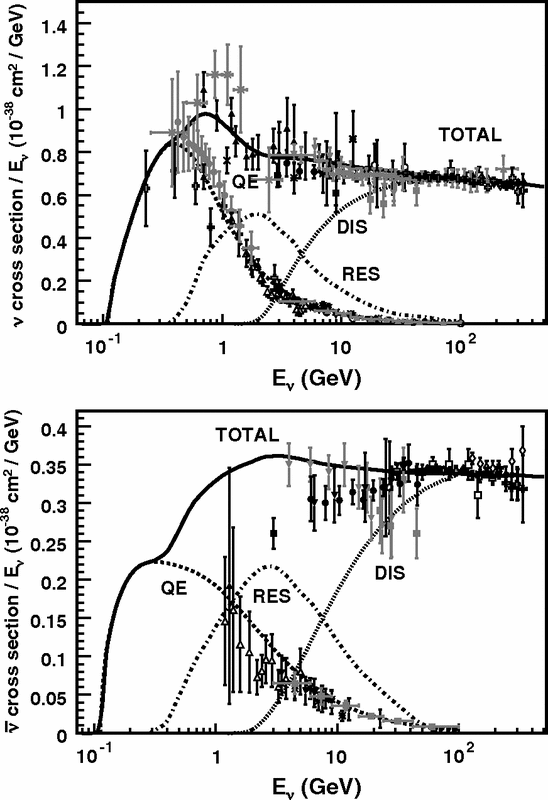
\includegraphics[width=0.48\textwidth,keepaspectratio]{neutrino_nucelon_crosssections.png}
  \end{center}
  \caption{Total inclusive cross-section is plotted above as a function of energy along with individual cross-sections for different interaction channels. Above a few tens of GeV, it's clear that deep inelastic scattering begins to dominate \cite{2012RvMP...84.1307F}.}
  \label{fig:neutrino_scattering}
\end{wrapfigure}

In the elastic (NC) or quasi-elastic (CC) scenario, an incoming neutrino will scatter off of the nucleon as a whole imparting some of its energy to the target. This is usually sufficient to eject the target nucleon and in some cases additional nucleons from the nucleus. The CC scattering is referred to as quasi-elastic due to the fact that it requires the conversion of the target proton(neutron) into a neutron(proton) to ensure charge conservation. This type of scattering does not probe the internal constituents of the nucleus (quarks and gluons collectively referred to as partons). The absolute cross-section, however, will depend heavily on nuclear properties of the target atom.

The most important neutrino-matter interaction in IceCube is that of deep inelastic scattering. As Figure \ref{fig:neutrino_scattering} shows, it is far and away the dominant mode of interaction for neutrinos above the threshold energy for detection.

\begin{figure}[ht]
  \begin{center}
    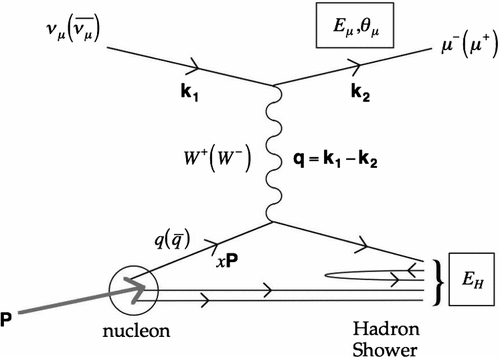
\includegraphics[width=0.7\textwidth,keepaspectratio]{dis.png}
  \end{center}
  \caption{Feynman diagram of a $\nu_{\mu}$ undergoing deep inelastic scattering with a nucleon via charged-current interaction. A large momentum exchange through a charged $W$ boson leads to breakup of the nucleon.}
  \label{fig:dis_scattering}
\end{figure}

\subsection{Propagation of Interaction Products}
The products leftover from high-energy neutrino-nucleon interactions are generally very energetic as well. These particles will subsequently undergo many forms of energy loss and possible decay as they travel through a potential detection medium. In a given interaction, the total light yield and its spatial extent are contingent on the products of the interaction. The products themselves are ultimately determined by both the flavor of the primary neutrino and whether the neutrino interaction was of the charged- or neutral-current variety. This section will focus on how these secondaries interact and produce light and how that light propagates through glacial ice, the detection medium of IceCube.

For neutrinos of sufficient energy to be seen by IceCube, scattering with nucleons in the ice via either neutral or charged boson exchange will result in the breakup of the nucleon target.
%% Hadronic Cascade
%% EM cascade from tau and e-
%% track produced via muon
\section{Flavor Oscillations}
The process in which the lepton flavor of a given neutrino can change during its propagation is one of the particles more intriguing properties. The unexpected observation of neutrino oscillations indicated that the neutrino, which was initially thought to be massless under the Standard Model, must actually have some non-zero mass after all. Recently, many experiments have studied this phenomenon with high precision in hopes of accurately determining the mass-splitting of the neutrino eigenstates as well as if neutrinos undergo CP violation. While the analysis being presented is in no way suited to studying the oscillation phenomenon, how the results are interpreted is very much dependent on how the modeled neutrino flavor ratio for a source evolves from its origin to its arrival at Earth. Thus, this section will describe in short detail the oscillation process over astronomical baselines and through the Earth, the scenarios most applicable to IceCube.


\chapter{Neutrino Astronomy}

\section{Motivation}


%% Illustration of different messengers
%% Cosmic ray -- Neutrion Connection

\section{Detection Methods}

The primary method for the detection of high-energy neutrinos is through observation of Cerenkov light produced by interaction secondaries in a transparent medium. Events can be detected either by surrounding a detection volume with light detectors (as is the case for Super-Kamiokande) or by placing the detectors within the detection medium itself (e.g. IceCube, ANTARES).
\chapter{Neutrino Sources}


\section{Active Galactic Nuclei}

\section{Gamma-ray Bursts}

%% Fireball model, neutrino production in jets
%% subphotospheric model

\begin{figure}[ht]
  \begin{center}
    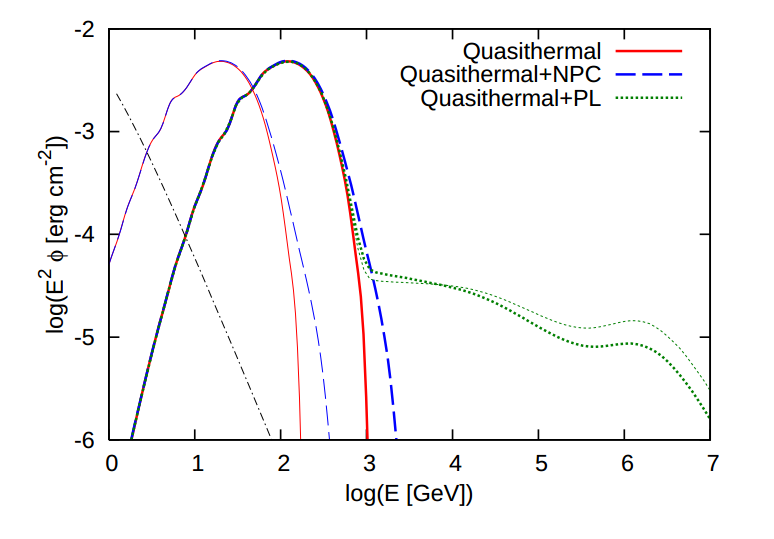
\includegraphics[width=0.85\textwidth,keepaspectratio]{SubPhotoFluence.png}
  \end{center}
  \caption{Energy Fluence of $\nu_{\mu}$ and $\bar{\nu}_{\nu}$ from high-luminosity GRB at a redshift of z=0.1 \cite{2013PhRvL.111m1102M}}
  \label{fig:subphotospheric_nus}
\end{figure}

\section{Core-Collapse Supernovae}
The detection of several neutrino events in temporal coincidence with supernova 1987A marked the first detection of an extra-solar neutrino source. Neutrino events were observed in three separate detectors a few hours prior to the optical observation. Such an observation was made possible by the close proximity ($\sim$50 kpc) of the progenitor located within the Large Magellanic Cloud. Detection of these events confirmed the theoretical prediction of an enormous liberation of energy in the form of neutrinos during the collapse of the core of a massive star.


%% neutrino production from neutron conversion, SN1987A
%% Too low energy in IceCube, but SNDAQ
\begin{wrapfigure}{r}{0.5\textwidth}
  \begin{center}
    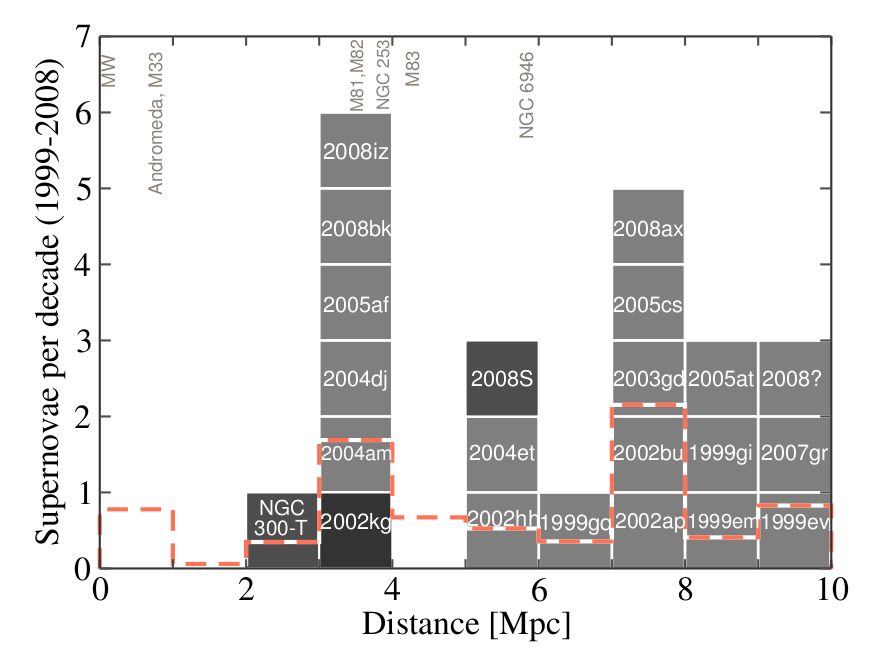
\includegraphics[width=0.48\textwidth,keepaspectratio]{NearbySNCatalogue.png}
  \end{center}
  \caption{Observed SNe within 10 Mpc in the years 1999-2008 \cite{2011PhRvD..83l3008K}}
  \label{fig:local_ccsne}
\end{wrapfigure}

\section{Choked Gamma-ray Bursts}



\chapter{Detector}
\section{IceCube and IceTop}
The IceCube Neutrino Observatory is a km$^{3}$-scale neutrino detector located deep within the glacial ice of the Antarctic ice sheet at the geographical South Pole. This location provides IceCube with a pristine detection medium in addition to mechanical support for the entirety of the array. The detector consists of 5,160 light sensors known as digital optical modules (DOMs) which are distributed along 86 cables (referred to as strings) that supply power and provide communication to the surface. Each cable is instrumented with 60 DOMs spaced 17 meters apart starting at 1450 meters below the surface and terminating at 2450 meters below. An inter-string spacing of 125 meters on average results in a total instrumented volume of approximately 1 km$^{3}$. Figure \ref{fig:icecube} provides a schematic illustrating the detector geometry.

\begin{figure}[ht]
  \begin{center}
    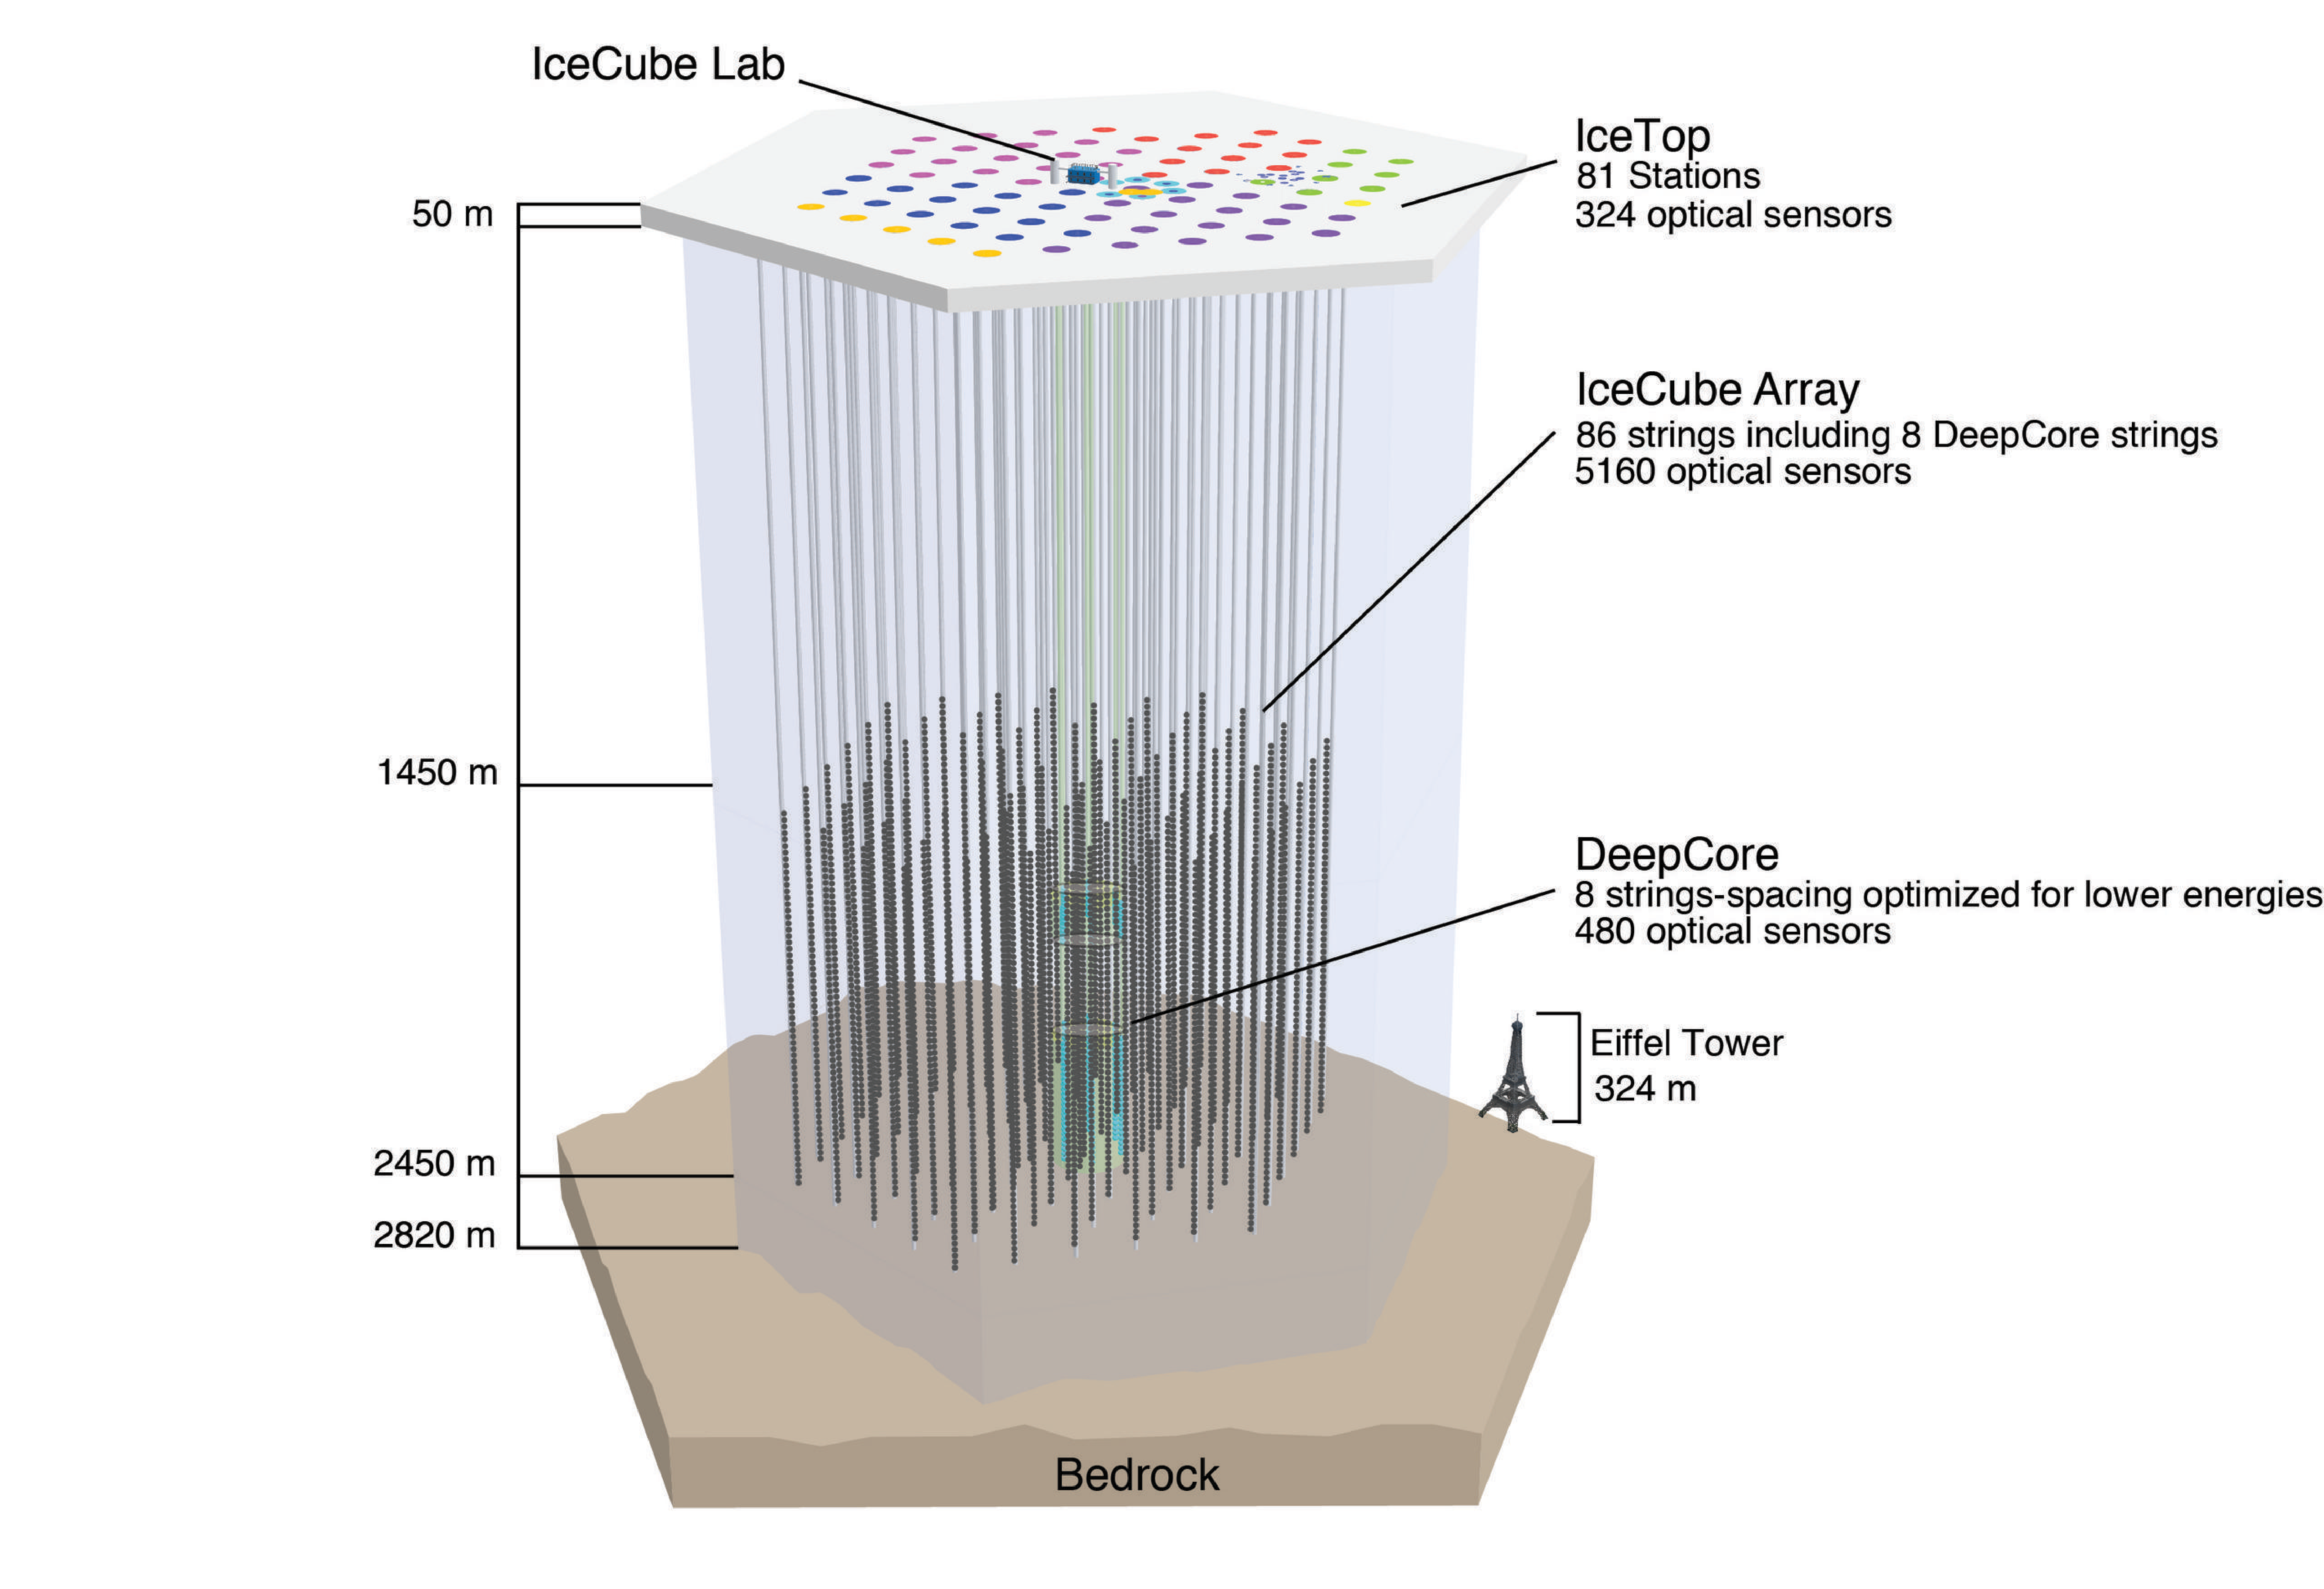
\includegraphics[width=1.0\textwidth,keepaspectratio]{ArrayWSeasonsLabels.pdf}
  \end{center}
  \caption{Diagram of the IceCube Neutrino Observatory (Courtesy of the IceCube Collaboration).}
  \label{fig:icecube}
\end{figure}

Installation of the IceCube strings took place over several years and required the use of a specialized hot-water drill. In the deployment process, the hot-water drill is used to bore through the ice leaving a water-filled column in which the string and its attached DOMs are lowered. The water column subsequently freezes the cable and all DOMs in place rendering them completely inaccessible from the surface. The deployment of the first IceCube string occurred on January 29th, 2005. The remaining strings were deployed over the next five summer seasons resulting in data seasons of different detector shapes and size. The final string was deployed on December 18, 2010 giving IceCube its ultimate 86-string configuration.

%%% IceTop

In addition to the detectors installed deep in the ice, there are also 81 surface detector stations (each station consisting of two tanks) at the surface. These tanks, which utilize two of the same light-sensing DOMs as IceCube, comprise the IceTop surface array. The DOMs in these tanks, which are also frozen in place, look for Cerenkov radiation produced by cosmic ray air shower secondaries in the tank ice. By examining the arrival time of charged particles from the shower front, the direction of cosmic rays incident at Earth can be determined. The spatial extent of the shower as well as the total charge deposition in tank PMTs allows for accurate estimation of the energy of the primary cosmic ray. Data produced from IceTop is used to study cosmic ray composition, spectra, and anisotropy.

Due to the spatial relation of both IceTop and IceCube, they are able to complement the capabilities of each other quite nicely. IceTop's primary purpose is to study air shower physics, but it also serves as a veto for downgoing atmospheric muons and neutrinos in IceCube. This is particularly useful in the search for highly energetic neutrinos of astrophysical origin such as the events reported in \cite{2013Sci...342E...1I} and \cite{2014PhRvL.113j1101A}. Any downgoing events found by these searches that is accompanied by a causually connected air shower signal in IceTop is immediately identified as atmospheric in origin. Alternatively, the background muons detected in IceCube can be used for more detailed study of air shower composition and energy in IceTop analyses. For more detailed information on the physics goals and detection capabilities of IceTop, see \cite{2013NIMPA.700..188A}.


\section{DeepCore}

DeepCore \cite{2012APh....35..615A} is a sub-detector deployed in tandem with IceCube between 2009 and 2010 primarily designed to lower the energy threshold of IceCube. The array consists of eight infill strings located in the center of the IceCube detector in addition to the first layer of surrounding standard IceCube strings. This configuration gives DeepCore three layers of IceCube strings to use as an active veto for the primary background of atmospheric muons. In order to improve detector response to lower energy neutrinos, $\mathcal{O}$(10-100 GeV), the infill strings of DeepCore have a much closer inter-string separation (~42 m) and have 50 DOMs spaced 7 m apart deployed deep in the ice between 2100 m and 2450 m. This denser instrumentation allows for better timing and spatial resolution of charged secondaries produced in neutrino interactions. Additional sensitivity to lower energies is gained throug the use of the newer Hamamatsu R7081MOD model PMT in the infill string DOMs as opposed to the standard Hamamatsu R7081-02 used in IceCube. This model boasts higher quantum-efficiency in the photocathode for photons at typical Cernkov wavelengths ($\lambda \sim 400$ nm). In-ice measurements of the high quantum efficiency (HQE) DOMs showed a 35$\%$ increase in sensitivity to Cerenkov light with respect to the standard IceCube DOMs \cite{2012APh....35..615A}.

The depth selected for deployment of the DeepCore DOMs was determined via examination of the ice properties previously mapped by both the Anatarctic Muon and Neutrino Detector Array (AMANDA) \cite{2006JGRD..11113203A} and pre-existing IceCube configurations \cite{2013JGlac..59.1117.}. These investigations into the optical properties of the ice revealed that the deepest ice ($\leq$ 2100 m) had superior optical qualities with respect to the ice closer to the surface. Additionally, it was determined that a layer of high dust concentration in which light is scattered and absorbed to a much higher degree exists at a depth of 2000-2100 m. The eight infill strings also have a section of 10 DOMs with 10 m spacing located just above the dust layer. These DOMs form a veto cap to further increase the detection probability and rejection of directly down-going muons. Figure \ref{fig:DeepCoreSchematic} shows the distribution of DeepCore DOMs and the spacing and orientation of the DeepCore strings with respect to IceCube as a whole.

\begin{figure}[ht]
  \begin{center}
    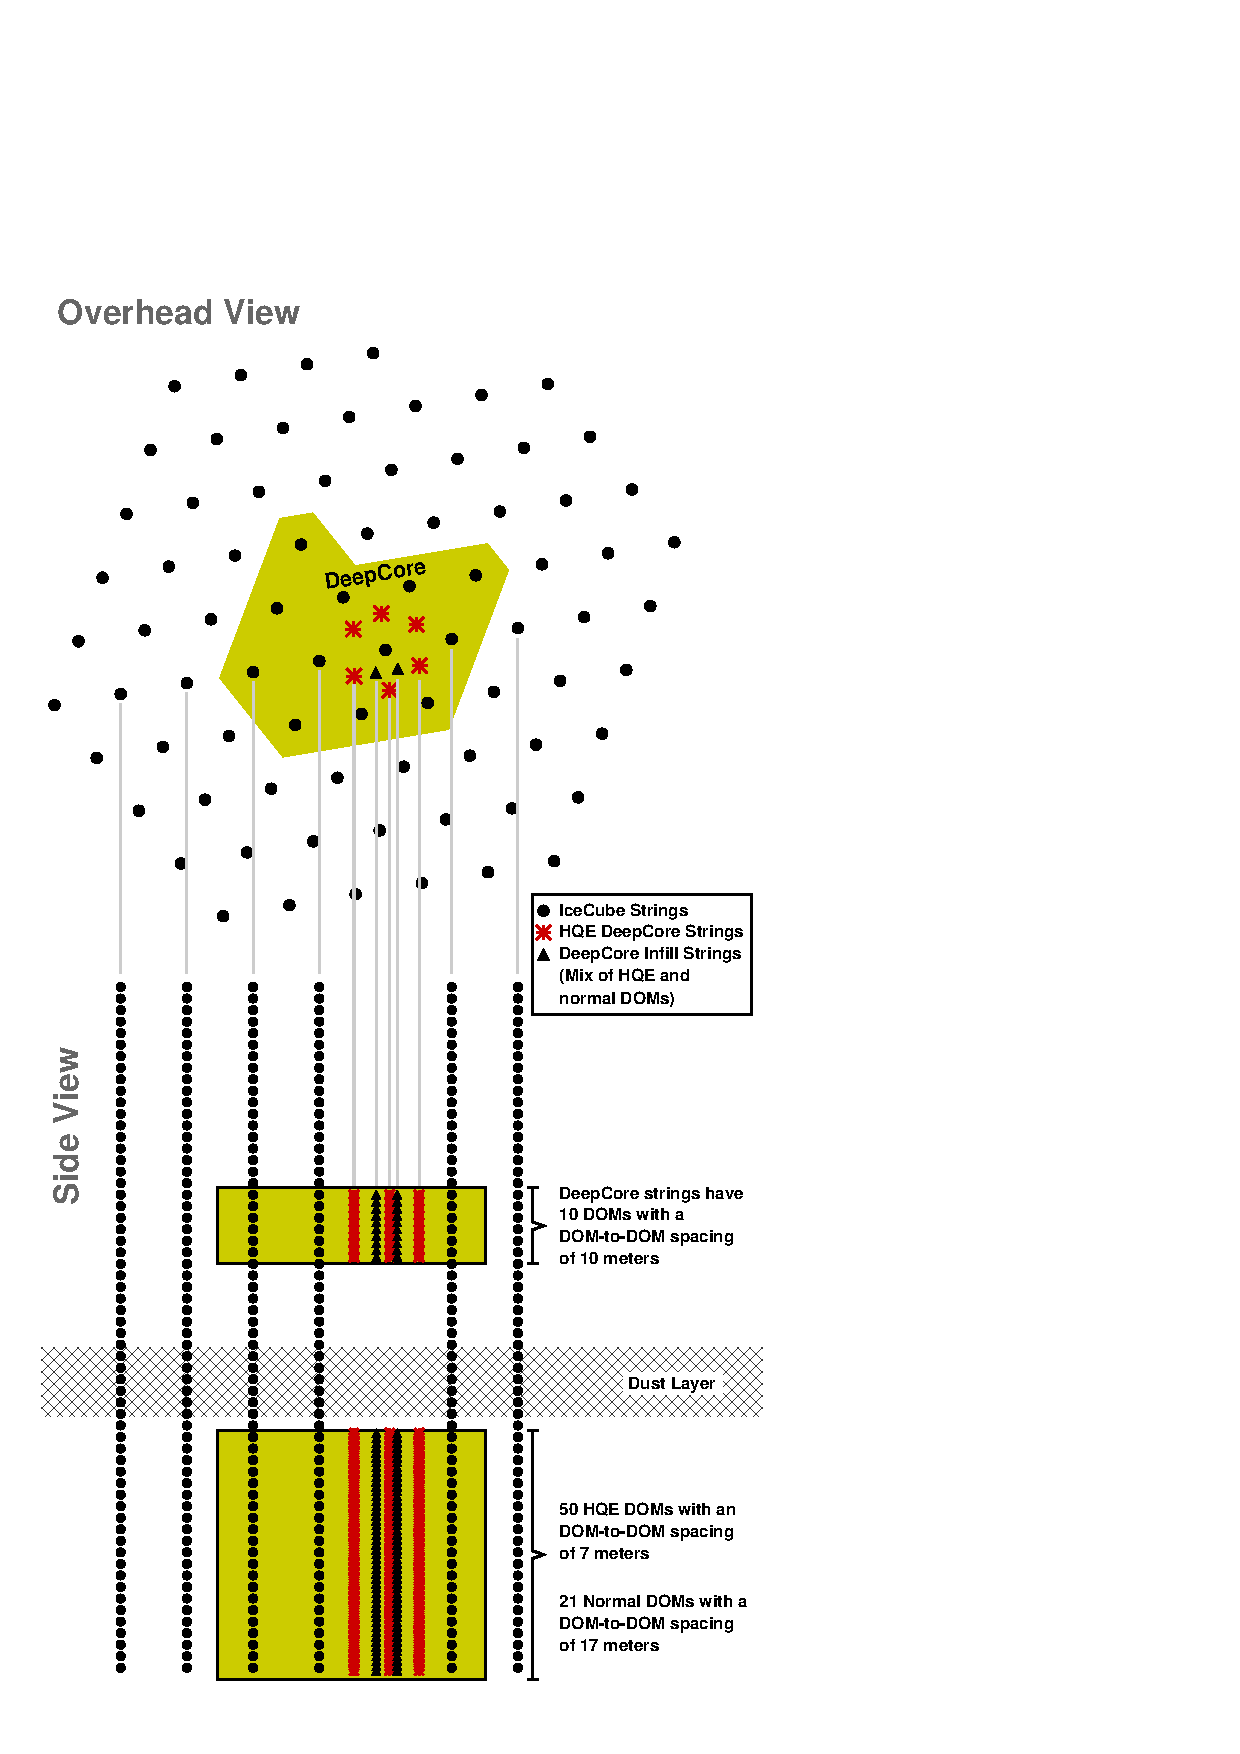
\includegraphics[width=0.7\textwidth,keepaspectratio]{IC86EDC_DeepCoreDiagram.pdf}
  \end{center}
  \caption{Top down and side-view diagram of DeepCore. The side-view shows the difference in DOM distribution for the infill strings and their relation to the dust layer \cite{2012APh....35..615A}.}
  \label{fig:DeepCoreSchematic}
\end{figure}

%%% Physics in DeepCore
The primary physics goal of the DeepCore installation is to provide increased sensitivity for indirect dark matter searches by improving the IceCube detectors ability to resolve sub-100 GeV neutrino events. In this regard, it has been quite successful in establishing limits on the cross-sections of many WIMP (Weakly Interacting Massive Particle) dark matter models with the Sun \cite{2013PhRvL.110m1302A} and Milky Way \cite{2011PhRvD..84b2004A} as possible sources. The lowering of the detector's energy threshold has also made neutrino oscillation parameter measurements possible due to the high statistics provided by atmospheric neutrino events \cite{2013PhRvL.111h1801A}. Most importantly for the analysis presented in this thesis, however, is the improvement in effective area and resolution DeepCore provides for 30-150 GeV muon neutrinos. As this thesis will demonstrate, including these neutrino events into previously established IceCube point source analysis methods greatly improves IceCube's capability to discover transient events with soft spectra.
\section{Neutrino Events in IceCube}

In order to isolate the sparse neutrino events from the abundance of background cosmic ray muons, it is necessary to fully understand the nature of the detector response to neutrinos and neutrino secondaries interacting within the detector. Neutrinos that are sufficiently energetic to be detected by IceCube will undergo deep inelastic scattering with a nucleon target (see for more information on this process see section \textbf{2.1.1}). This process will either be charged-current (CC) or neutral-current (NC) depending on the nature of the boson exchange and the final lepton state. The hit topology of a given neutrino event in IceCube will depend upon the flavor of the neutrino ($\nu_{e}$, $\nu_{\mu}$, $\nu_{\tau}$) as well as the channel through which it interacts with a target nucleon in the ice.

In NC interactions of all flavors, a hadronic cascade is produced which yields a roughly isotropic distribution of light. Any spatial extent in the hadronic cascade particles will be much smaller than the DOM separation distance. Thus, the Cerenkov emission from these particles will appear to be a point source of light within the detector. This results in a spherical pattern of DOMs that register light from this type of interaction. The radius of DOMs which are able to detect light from the cascade is determined by the total energy deposited in the ice by the neutrino primary. Events with this hit pattern are referred to as cascades. An example event display for this type of interaction can be seen in Figure \ref{fig:cascade}.

\begin{figure}[ht]
  \begin{center}
    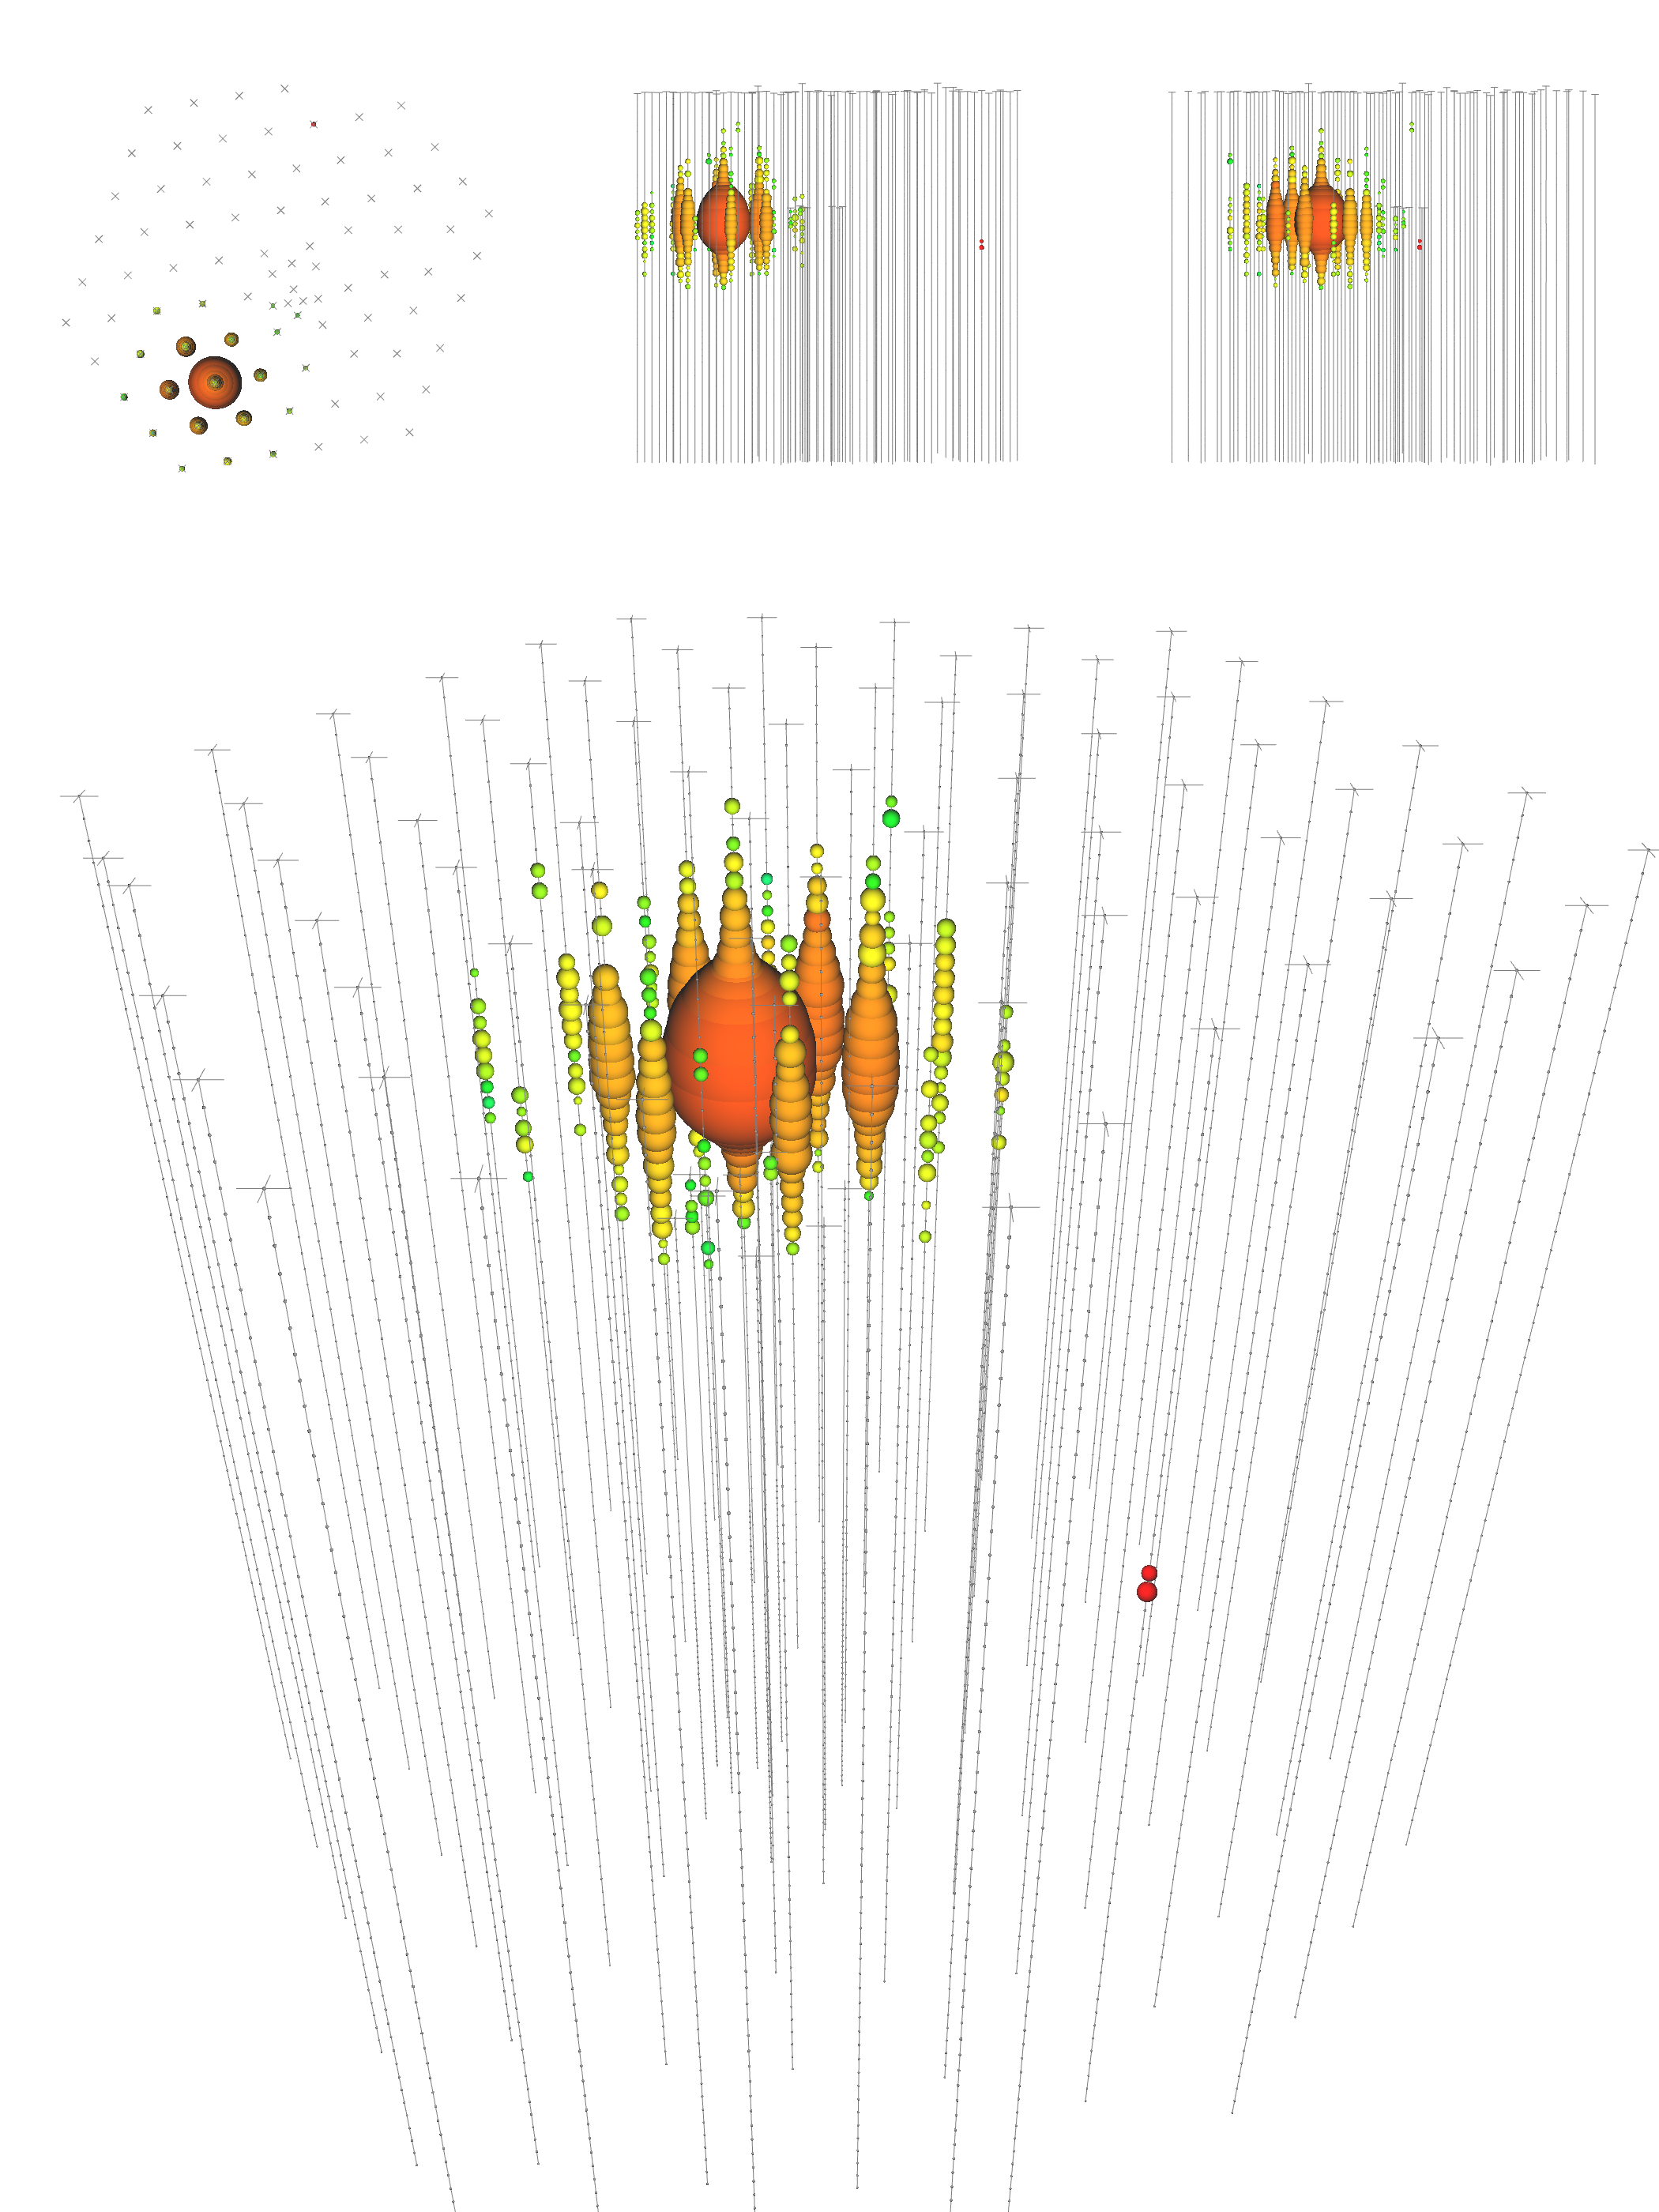
\includegraphics[width=1.0\textwidth,keepaspectratio]{hese_cascade_event.png}
  \end{center}
  \caption{A high-energy cascade event in IceCube with deposited energy of $210\pm^{29.0}_{25.8}$ TeV \cite{2013Sci...342E...1I}. The colored spheres represent DOMs that have registered light during the event. The size of the spheres are indicative of the total light received by the PMT on that DOM. The color denotes the timing of the hit with red corresponding to earlier times and blue corresponding to later times.}
  \label{fig:cascade}
\end{figure}

Whereas the resultant hit pattern for NC interactions is flavor independent, the event topology in CC interactions is determined primarily by the lepton flavor of the neutrino. In addition to a hadronic cascade, the CC interaction will also yield an energetic lepton corresponding to the flavor of the interacting neutrino. In the case of $\nu_{e}$ and $\nu_{\tau}$ CC interactions, the resulting hit pattern in IceCube will take the form of a cascade in a similar manner to the NC interactions. While the source of Cerenkov emission is no longer point-like, the length of electron and tau particle tracks is much shorter than the inter-DOM separation distance. Some marginal pointing can be achieved for these events, however, since the light produced in the hadronic and electromangetic cascades in these events is not totally symmetric. For sufficiently energetic $\nu_{\tau}$ events in IceCube, more exotic signatures are possible. These arise from the increased lifetime of the outgoing $\tau$ lepton resulting in two separate light-producing cascades that can be resolved separately either in space or time. As of the writing of this thesis, no events of this type have been observed in IceCube.

IceCube is designed specifically to be sensitive $\nu_{\mu}$ CC interactions due to superior pointing provided by long-lived muon tracks in the ice. Daughter muons from $\nu_{\mu}$ CC interactions can travel distances ranging from ~300 m ($E_{\nu_{\mu}}\sim 100$ GeV) to several kilometers ($E_{\nu_{\mu}}\geq 1$ TeV) \cite{2001PhRvD..63i4020I}. As these muons travel through the ice, they produce light in electromagnetic showers through both ionization and stochastic radiation losses. Because the muon is traveling faster than the speed of light in the ice ($n_{ice} \sim 1.3$), the Cerenkov light generated about the muon track will form a cone which is ultimately aligned with the original neutrino direction. This results in a linear hit pattern in IceCube DOMs, providing a clear signal with good directional information. Muon tracks with the highest contained length in the detector provide the best resolution due to their long lever arm and low kinematic angular difference with respect to the parent neutrino. An example of a track event from a high-energy contained event search is shown in Figure \ref{fig:track}.

\begin{figure}[ht]
  \begin{center}
    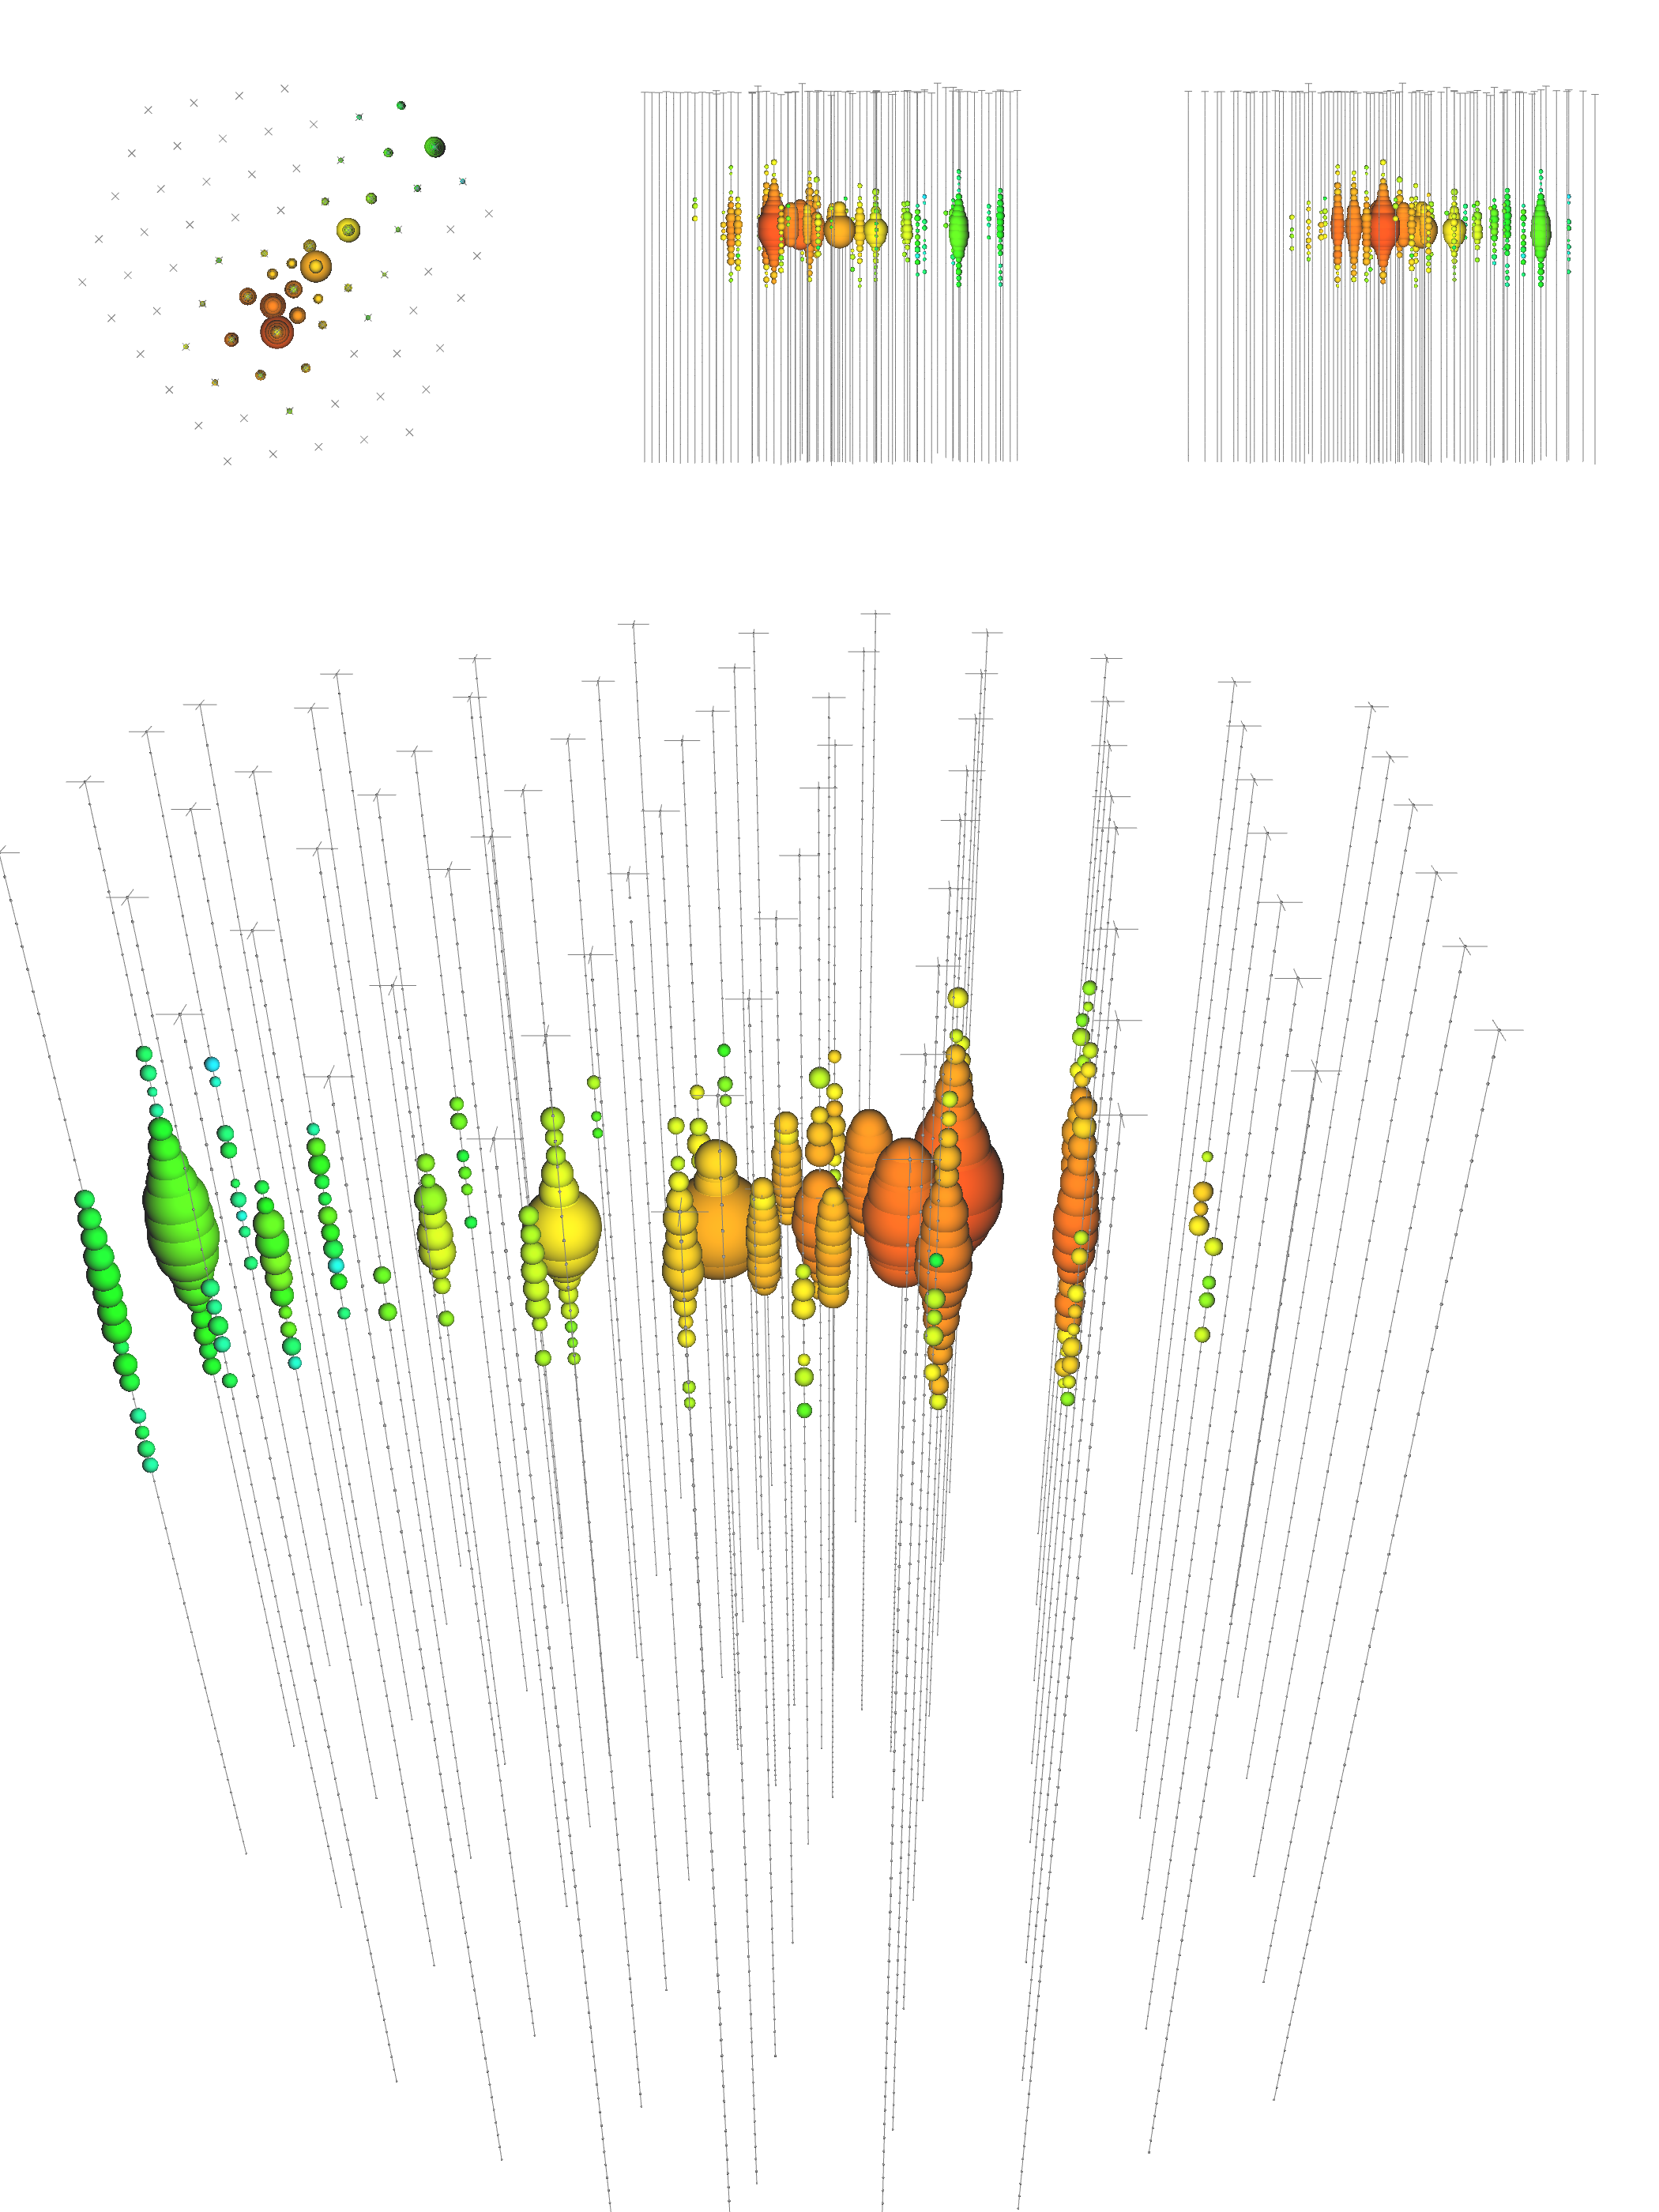
\includegraphics[width=1.0\textwidth,keepaspectratio]{hese_track_event.png}
  \end{center}
  \caption{A high-energy track event in IceCube with deposited energy of $71.4 \pm 9.0$ TeV \cite{2013Sci...342E...1I}. The colored spheres represent DOMs that have registered light during the event. The size of the spheres are indicative of the total light received by the PMT on that DOM. The color denotes the timing of the hit with red corresponding to earlier times and blue corresponding to later times.}
  \label{fig:track}
\end{figure}


\chapter{Data Acquisition}
Maintaining smooth and efficient data acquisition for a detector consisting of such a large number of sensors presents a formidable challenge. Reconstructing physics events within the detector requires accurate timing of signals received by individual sensors coupled with a high degree of synchronization among all detection elements. In this section, a succinct description of the detection of the light-yield from particle interactions in the ice and the subsequent processing of that data is given. The reader interested in a much more thorough account is encouraged to consult the summary by Abbasi et al. \cite{2009NIMPA.601..294A}. 

\section{The Digital Optical Module}
The essential component of the IceCube detector is the DOM. Each of these sensor units contains a Hamamatsu R7081-02 25 cm photo-multiplier tube (PMT), attached digitizing electronics, and LED flashers all housed within a glass pressure vessel \cite{2006NIMPA.567..214H}. A penetrator cable breaches the pressure vessel to connect the DOM electronics to the supporting string cable enabling DOM-to-DOM as well as DOM-to-surface communications. Absolute quantum-efficiency measurements were made for all DOMs prior to deployment in the ice. In order to estimate how the efficiency might change after freeze-in, studies on the efficiency of DOMs at typical in-ice temperatures were performed in labs at IceCube member institutions. 

%%Flasher Runs

%% Mainboard Suite

\begin{figure}[ht]
\centering
\begin{minipage}[b]{0.45\linewidth}
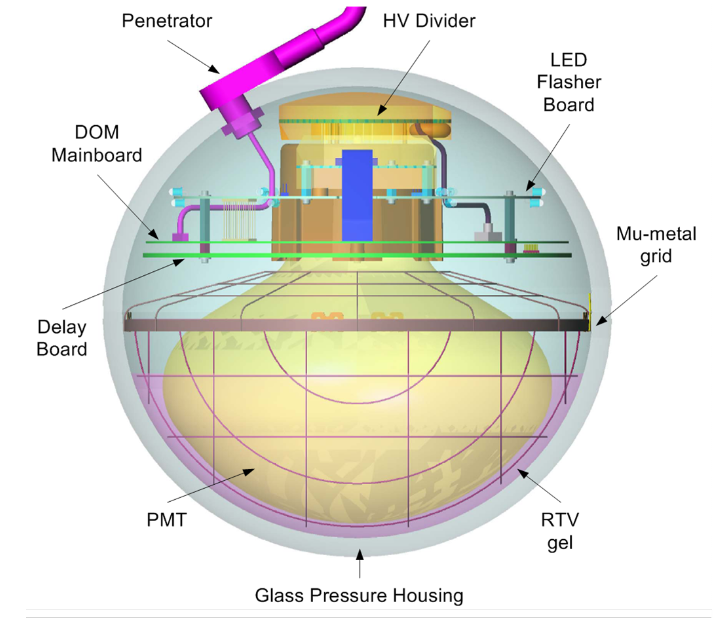
\includegraphics[width=0.95\textwidth]{DomSchematic.png}
\caption{Schematic detailing DOM structure \cite{2009NIMPA.601..294A}.}
\label{fig:domscheme}
\end{minipage}
\quad
\begin{minipage}[b]{0.45\linewidth}
\begin{center}
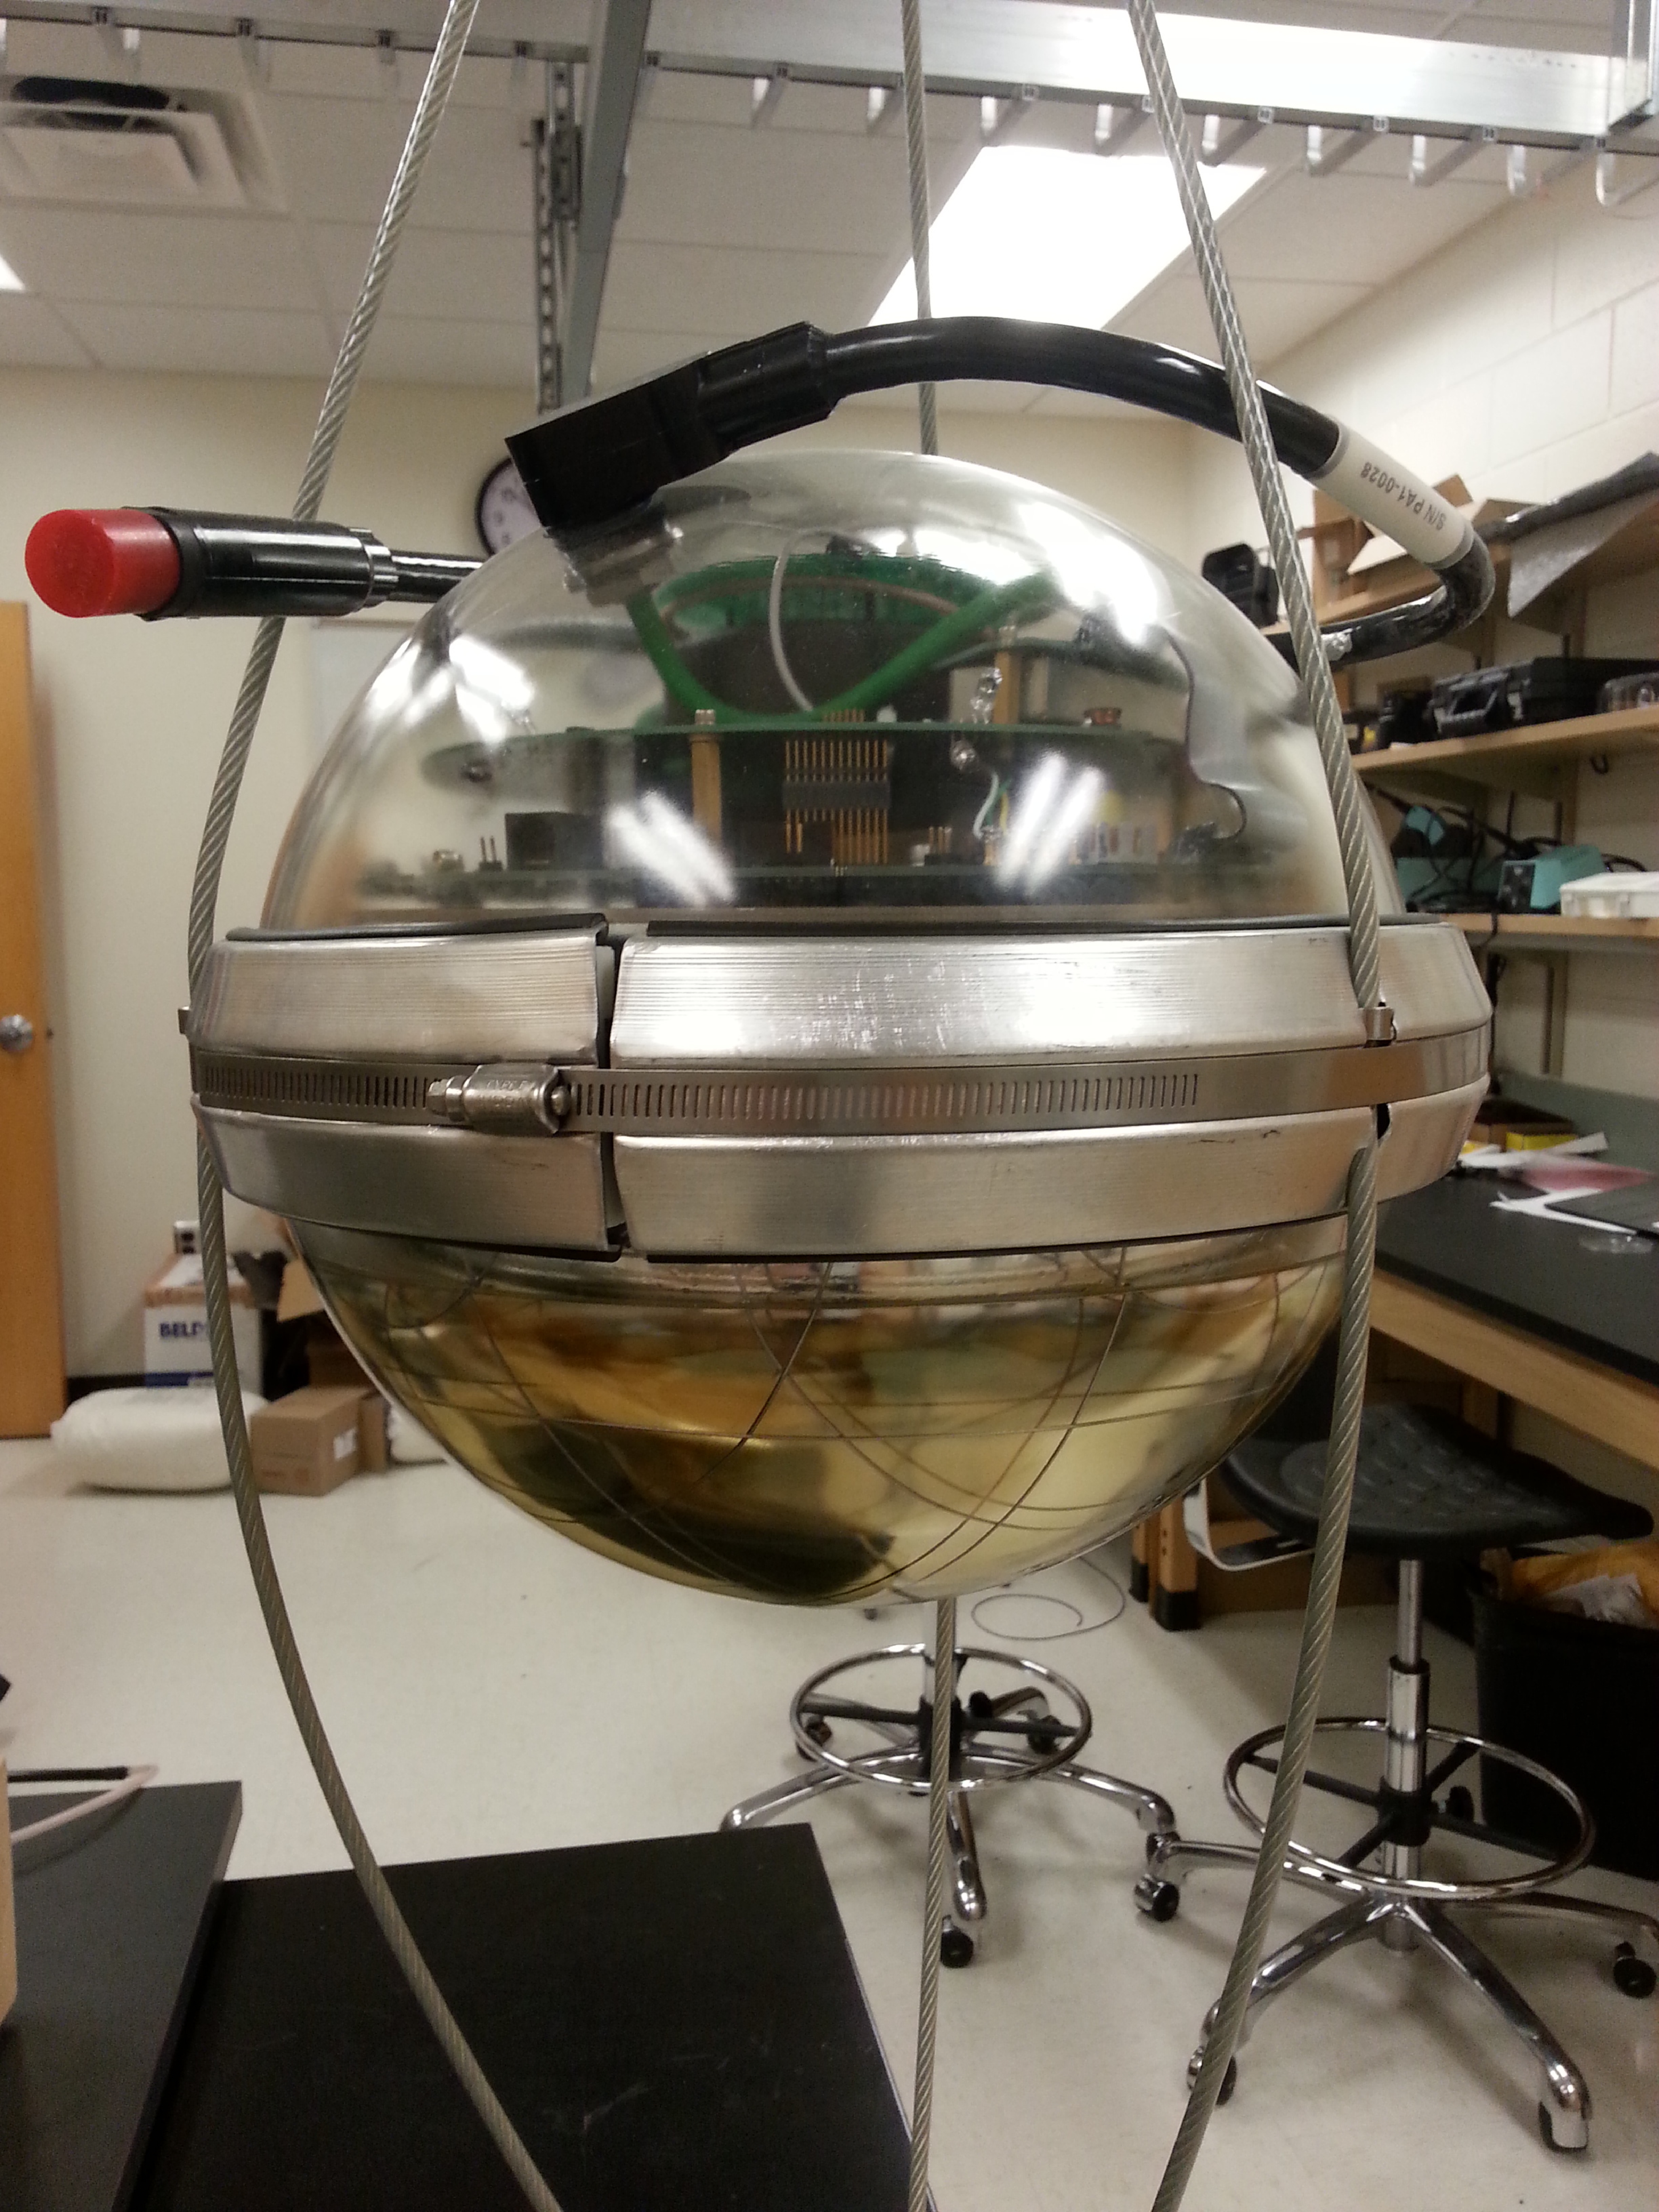
\includegraphics[width=0.75\textwidth]{LabDOM.pdf}
\end{center}
\caption{A fully assembled DOM supported by a cable harness.}
\label{fig:dompic}
\end{minipage}
\end{figure}


\section{Hit Generation}

All data acquisition begins with the registering and processing of photon hits in individual DOMs. Cerenkov photons from nearby passing charged secondaries are detected when they intercept the photocathode of the PMT on the underside of the DOM. This generates a small current pulse which is subsequently amplified 

\section{Data Synchronization}

\section{Triggering and Event Building}


\chapter{Event Selection}
A quick comparison between the rate at which atmospheric neutrinos trigger the IceCube and DeepCore detectors ($\sim$ 10 mHz) and the overall event rate ($\sim 3$ kHz) readily shows that the data generated by IceCube is very strongly dominated by background. This background is almost entirely due to energetic muons produced in cosmic ray air showers passing through the detector from above. Due to the large range of physics capabilities of the detector, many different filters exist to reduce the data volume and select out events of interest to specific analyses. Event selection for IceCube analyses generally consists of selecting the appropriate filter(s) for the expected signal followed by application of several iterations of cuts optimized to reduce background to an acceptable level while maintaining efficiency with respect to signal events.

%% Simulation

\section{Low-energy Channel}

Because of the primary focus of this analysis on a lower-energy event selection, the DeepCore-dominated low-energy filter stream is taken as input. Selecting only events which pass this filter reduces the trigger-level data rate of 3 kHz to a much more manageable 37 Hz. The low-energy filter attempts to select a relatively background free sample by selecting a detection volume about DeepCore that does not extend to edge of the detector. This allows optical sensors outside of the detection volume to serve as dedicated downgoing muon detectors. Events that have hits on DOMs outside the defined detection volume that are causally correlated with the hits inside the volume are able to be identified as background muons. A schematic representation of this filtering algorithm is shown in \ref{fig:}. 

%% Insert DeepCore Filter Pic

This filter actually consists of two separate streams which are differentiated by the definition of which DOMs comprise the detection (or fiducial) volume and which DOMs are treated as belonging to the veto region. Inclusion of this additional branch using the relaxed veto allows for increased acceptance of higher-energy upgoing muon neutrino events that may be cut by the more stringent definition. The acceptance rate for the standard and relaxed veto filters is 17.25 Hz and 23.3 Hz respectively. The end result is a reduction in the trigger level data rate of nearly two orders of magnitude yielding a much more manageable data sample on which more advanced background reduction techinques can be applied.

\section{Analysis Specific Cuts}

\subsection{Veto Cuts}

\subsection{Quality Cuts}

\subsection{Boosted Decision Tree}


\section{Event Reconstruction}
An accurate reconstruction of neutrino events in the data sample is critical for optimal performance of any pointing analysis. During the event selection process several iterations of reconstructions are performed so that downgoing muons from cosmic rays can easily be identified. 

\begin{figure}[ht]
\centering
\begin{minipage}[b]{0.45\linewidth}
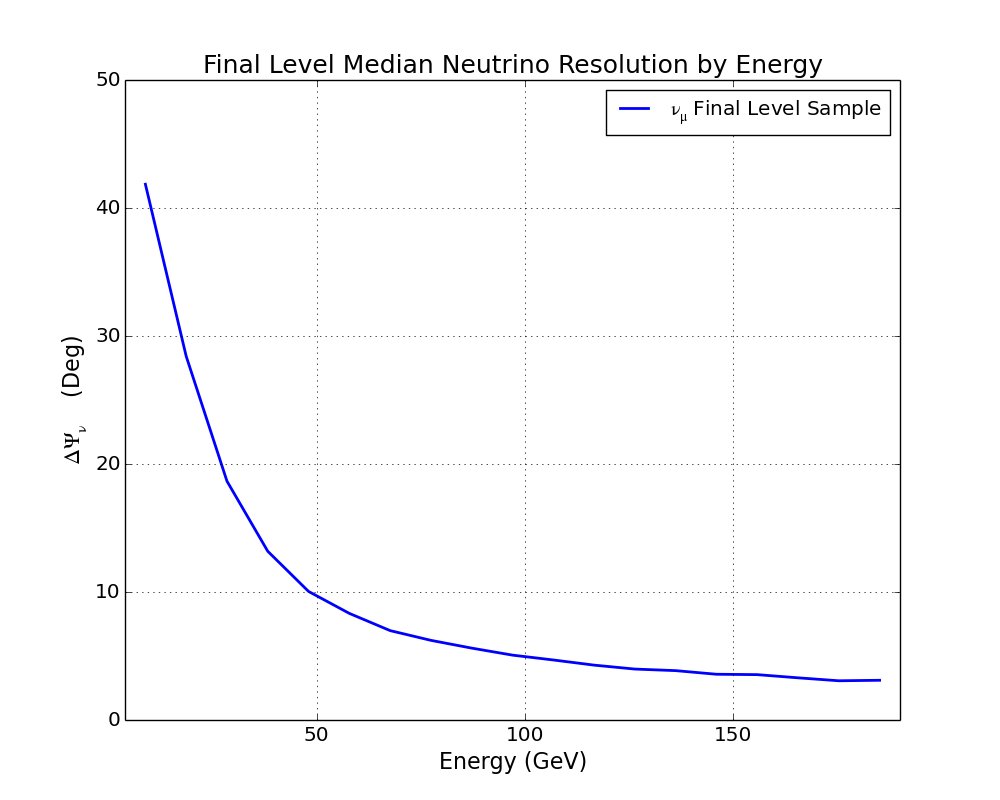
\includegraphics[width=0.95\textwidth]{FinalLevel_NeutrinoResolutionByEnergy_JustGENIE.png}
\caption{Median event resolution as a function of energy for simulation events passing all cuts.}
\label{fig:EventSampleRes_Energy}
\end{minipage}
\quad
\begin{minipage}[b]{0.45\linewidth}

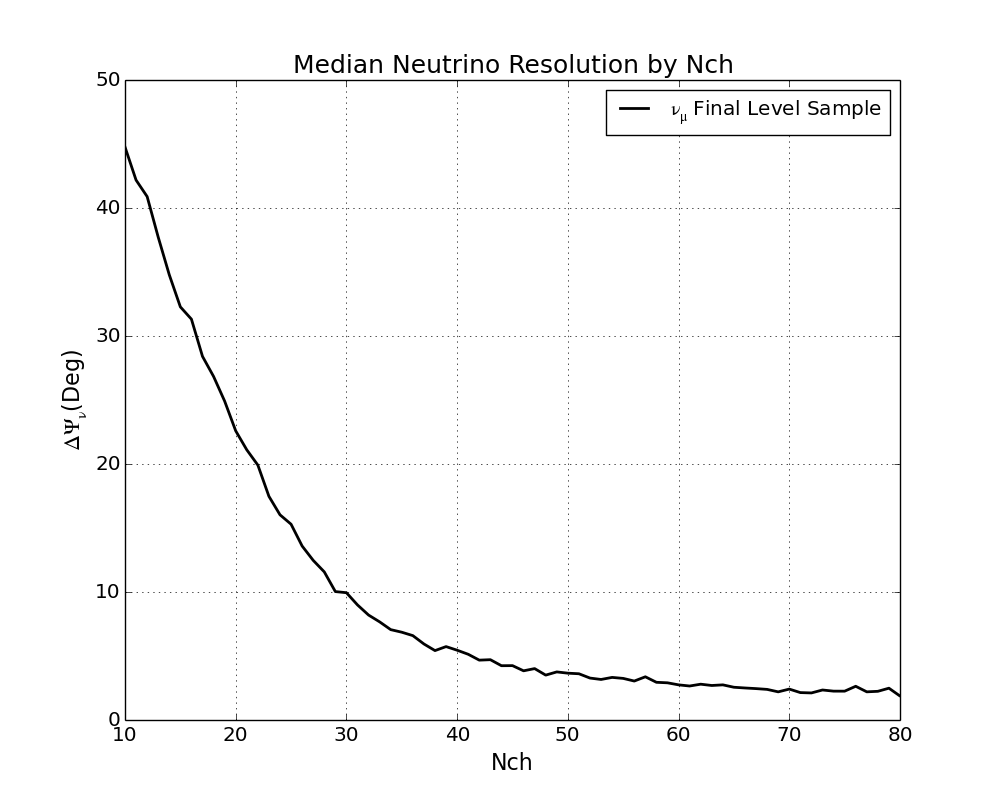
\includegraphics[width=0.95\textwidth]{GENIE_FinalLevel_NeutrinoResolutionByNch.png}

\caption{Median event resolution as a function of number of hit DOMs for simulation events passing all cuts.}
\label{fig:EventSampleRes_Nch}
\end{minipage}
\end{figure}


\section{Final Level Data}
After all cuts have been applied, we are left with a sample of 22,040 events during the observation period with an expected neutrino 'purity' of about 90$\%$. The bulk of these events are neutrinos of atmospheric origin and they represent the strongest background for the analysis.
\begin{table}[h]
\caption[Final level data rate.]{Summary of final level event rates in mHz. The amtospheric muon and neutrion rates are estimated through the use of Monte Carlo simulation (MC).\label{tab:event_rates}}
\begin{center}
\begin{tabular}{|l|r|}
  \hline
 \textbf{Event Type} &\textbf{ Rate (mHz)} \\
\hline
Cosmic ray $\mu$ & 0.065 \\
Atmospheric $\nu_{\mu}$ & 0.94 \\
Total MC & 1.001 \\ \hline
Actual Data     & 0.774 \\ \hline
\end{tabular}
\end{center}
\end{table}

%%% Insert Table for final level rates
%%% Refer to App. A for Pictures of Final Level Distributions

\begin{figure}[ht]
  \begin{center}
    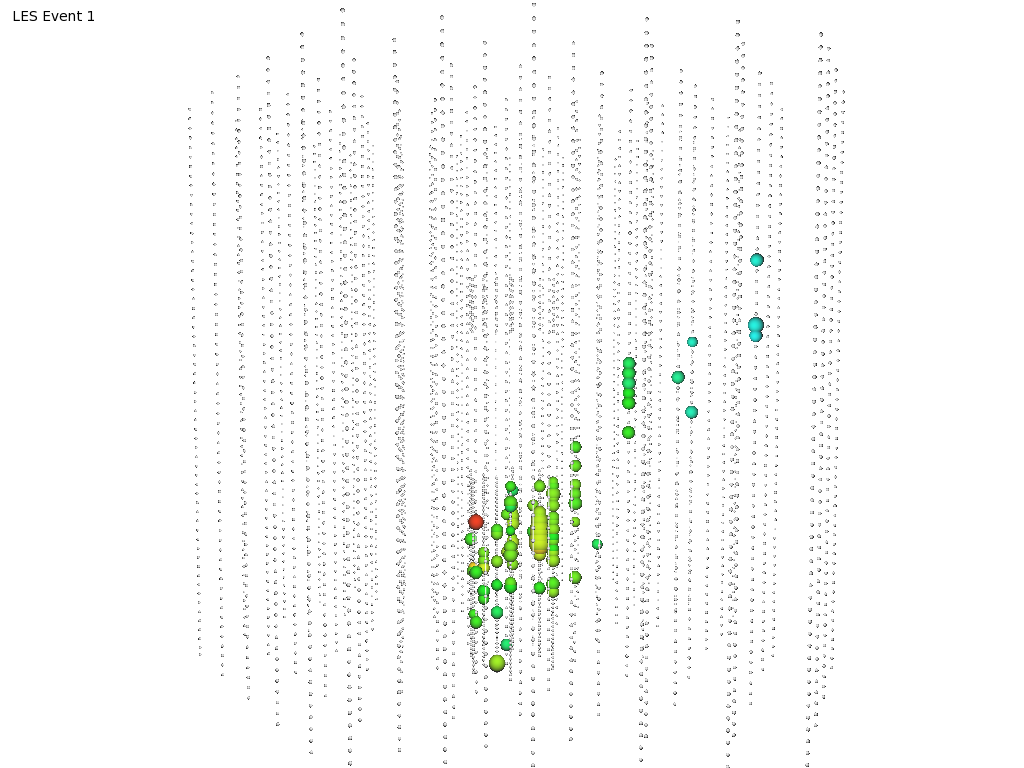
\includegraphics[width=1.0\textwidth,keepaspectratio]{LESEventForThesis.png}
  \end{center}
  \caption{Event display for a final level neutrino track event originating in DeepCore. The colored spheres represent DOMs that have registered a hit during the event. The size of the spheres are indicative of the total light received by the PMT on that DOM. The color denotes the timing of the hit with red corresponding to earlier times and blue corresponding to later times.}
  \label{fig:LESEventFinal}
\end{figure}


\chapter{Analysis Method}
%% Brief description of use of a time dependent search method
The analysis presented in this thesis makes use of both directional and timing information from the final level event dataset. The techniques that are used in this analysis have been applied to other IceCube event selections in a similar fashion. As of yet, these time-dependent searches focused on IceCube events have yet to find any time-dependent neutrino sources of significance higher than background expectations \cite{}. A very thorough overview of the time-dependent likelihood analysis methods used in IceCube is given by Braun, et al. \cite{2010APh....33..175B}. The method detailed in the following section is mostly the same, but there are a few minor modifications made to the process to improve performance on a low energy event selection.


\section{Unbinned Likelihood Method}
The identification of a statistically significant astrophysical signal amongst a high number of background events can be a difficult problem in astronomy. Searches will typically make use of timing, directional, and occasionally reconstructed energy information from events to find clustering indicative of a true astrophysical source. In order to accomplish this task, one can construct probability density functions or PDFs representative of the expected event spatial, temporal, or energy distributions for both signal and background possibilities.

\begin{equation}
S_i(|\mathbf{x}_i-\mathbf{x}_s|,t_i,t_o,\sigma_w) = \frac{\kappa}{4\pi \sinh \kappa} \exp \left(\kappa \cos |\mathbf{x}_i-\mathbf{x_s}|\right) * \frac{1}{\sqrt{2\pi}\sigma_w} \exp \left(-\frac{(t_i-t_o)^2}{2 \sigma_w^2}\right)
\end{equation}


\begin{equation}
B_i(\mathbf{x}_i,t_i) = P_{BkgDec}\left(\mathbf{x}_i\right)\frac{P_{BkgAz}(\delta_i,\alpha_i)}{T}
\end{equation}

\begin{equation}
\mathcal{L}(\mathbf{x}_s,n_s,t_o,\sigma_w) = \prod P_i(|\mathbf{x}_i-\mathbf{x}_s|,n_s,t_i,t_o,\sigma_w)
\end{equation}

\begin{equation}
\log \lambda = \log \left(\frac{\sqrt{2\pi}\hat{\sigma}_w}{T}\frac{\mathcal{L}(\mathbf{x}_s,\hat{n}_s,\hat{t}_o,\hat{\sigma}_w)}{\mathcal{L}(n_s = 0)} \right)
\end{equation}


\section{Sky Scan}

The analysis performed is not a triggered search, and therefore it is necessary to examine the entire solid angle domain of the analysis for any possible transient sources. The difficulty in rejecting background muons at lower energies limits the analysis to up-going and horizontal events ($< 5^{\circ}$ above the horizon). Because of IceCube's location at the South Pole, this results in a search over all right ascension in a declination band ranging from -$5^{\circ}$ to $90^{\circ}$. The search method discretizes the northern portion of the sky into many bins. The coordinates of these bins serve as the location of a hypothetical flaring source to be tested. The fairly large median resolution of the event sample (see Fig. \ref{fig:EventSampleRes_Energy}) allows the size of the search bins to be set to a relatively coarse 2$^{\circ}$ by 2$^{\circ}$ in angular area. 

%% Insert Sky Map

\begin{figure}[ht]
  \begin{center}
    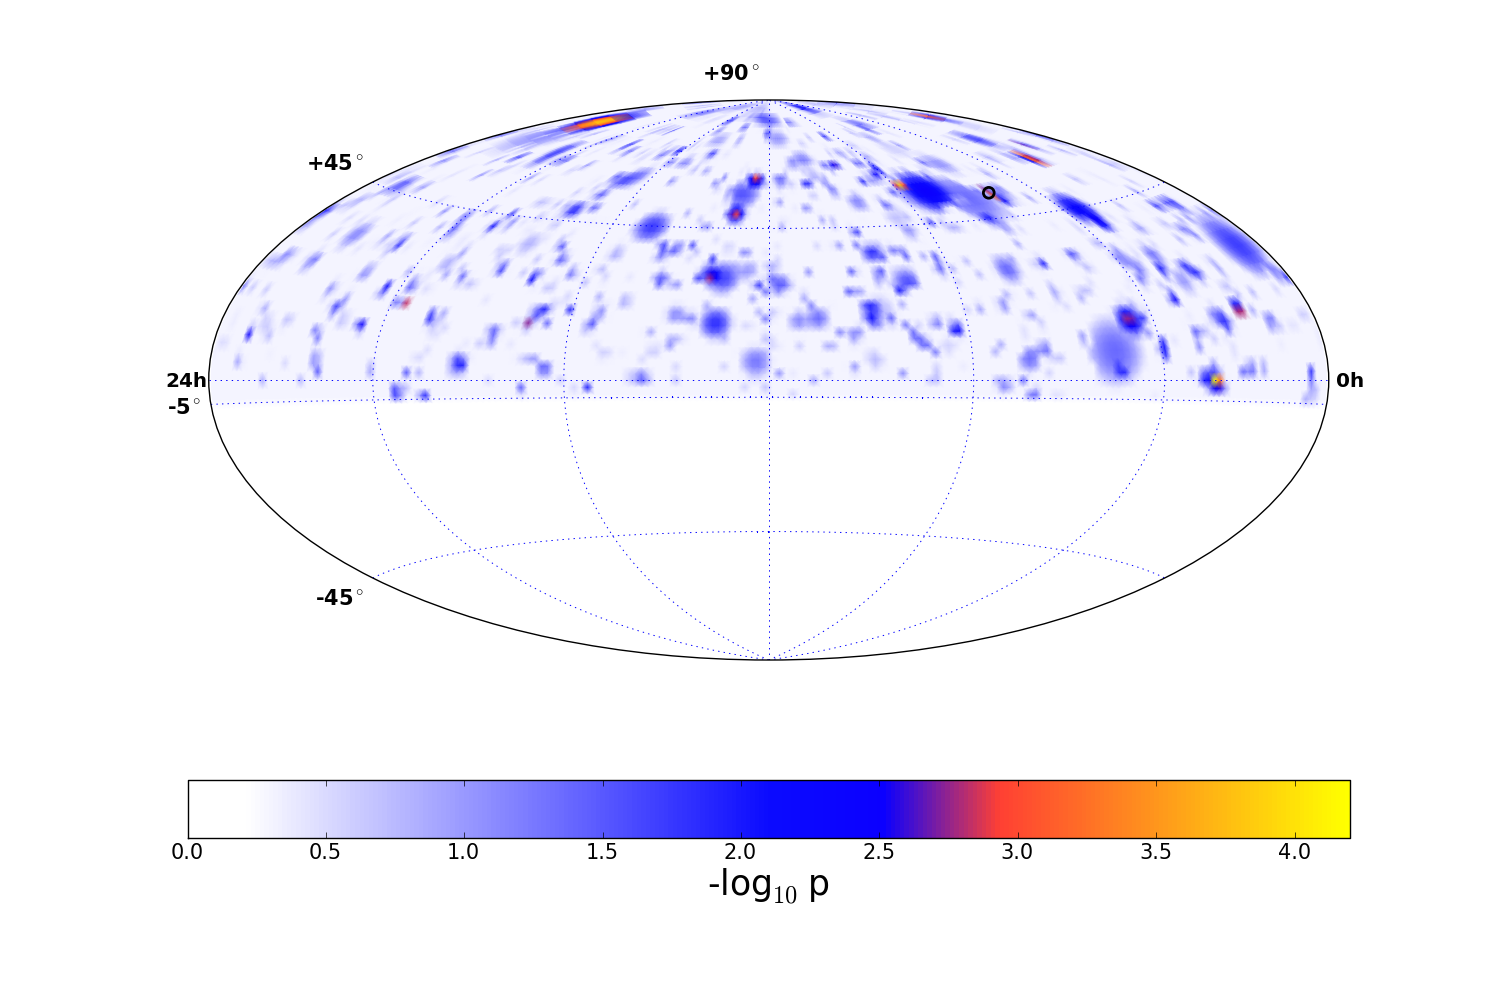
\includegraphics[width=1.0\textwidth,keepaspectratio]{NullMap996.png}
  \end{center}
  \caption{Randomized sky map of pre-trials p-values for best flares per bin. Random map generated by scrambling arrival times of real events. The black circle shows the location of the most significant flare found by the method. }
  \label{fig:NullTrialSkyMap}
\end{figure}

\section{Significance and Trials Factors}
In order to determine which bin has the most significant flare, we evaluate an estimated p-value based on the maximized test statistic $\lambda$ for that bin. The distribution of test statistic values for individual bins is not known \textit{a priori} however.
%% Insert Background Trials Best TS distribution

\chapter{Systematic Effects}
There are many systematic uncertainties that can affect the interpretation of the results of this analysis. The primary contributors to uncertainty being the \textit{in situ} scattering and absorption properties of the ice medium and the absolute quantum efficiency of the PMTs within the DOMs.

\section{Ice Properties}
The optical properties of the subsurface ice at the South Pole represent the most difficult systematic effect to adequately measure. This is largely due to the fact that this detection medium is inaccessible from the surface making direct measurement of the optical properties impossible.
\section{DOM Quantum Efficiency}

\chapter{Results}


%% Hottest Spot
%% SkyMap
\begin{figure}[ht]
  \begin{center}
    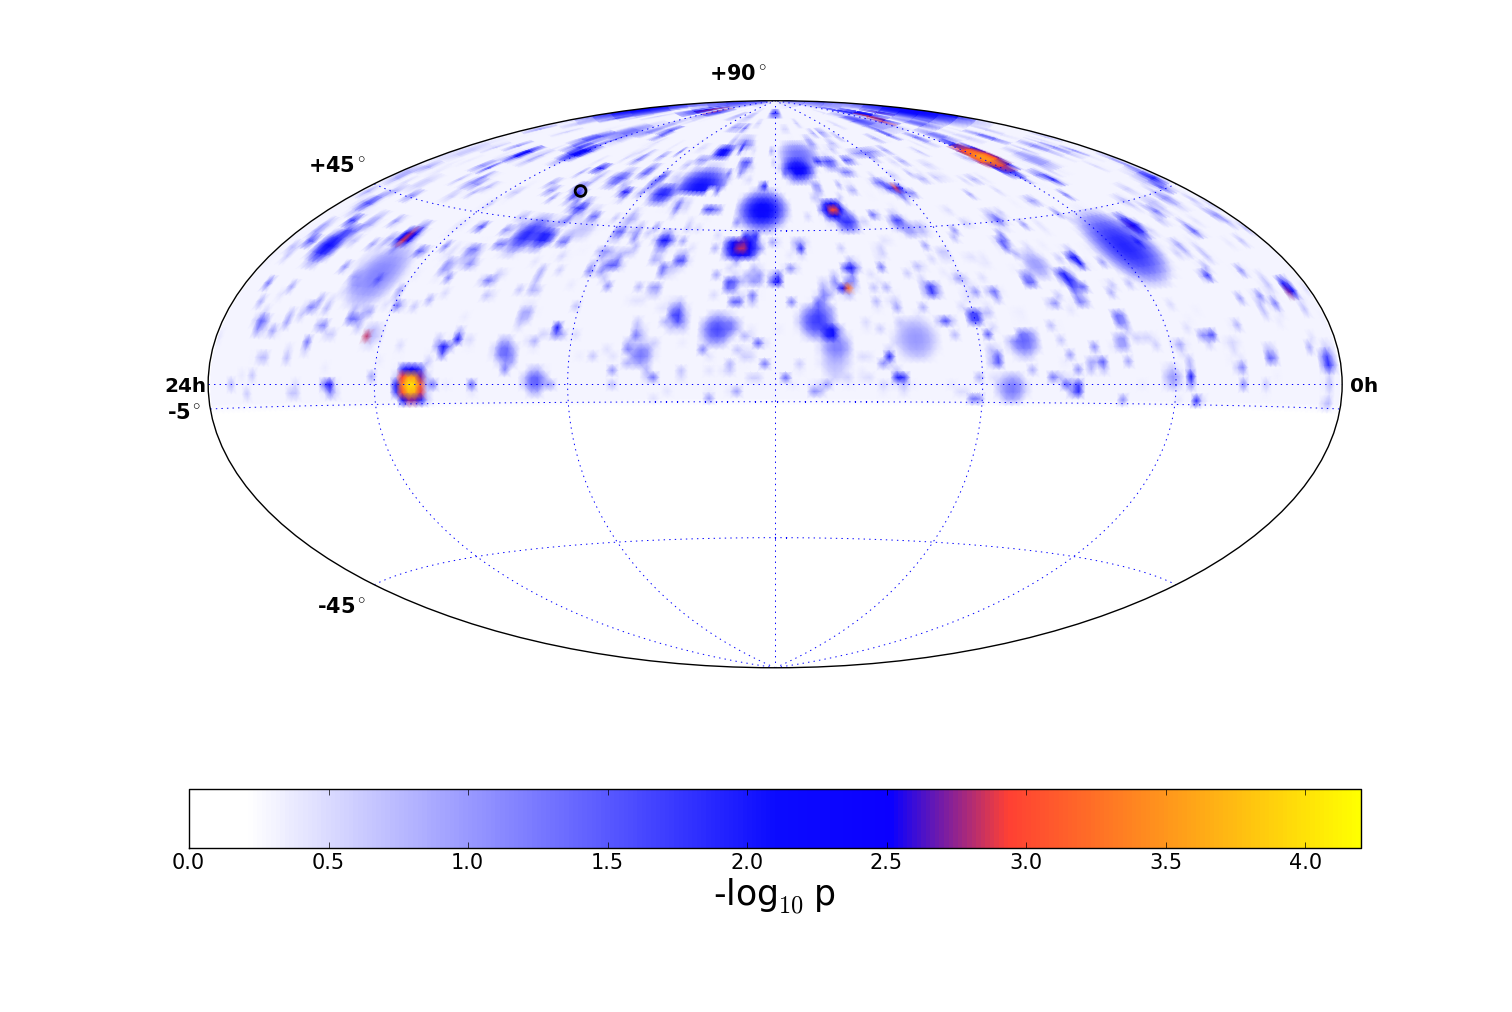
\includegraphics[width=1.0\textwidth,keepaspectratio]{RealResultSkyMap.png}
  \end{center}
  \caption{Sky map of pre-trials p-values for best flares per bin. The black circle identifies the location of the most significant flare found at RA = 268.75$^\circ$ and Declination = 54.25$^\circ$.}
  \label{fig:RealSkyMap}
\end{figure}

%% Post-trials p-value
\begin{figure}[ht]
  \begin{center}
    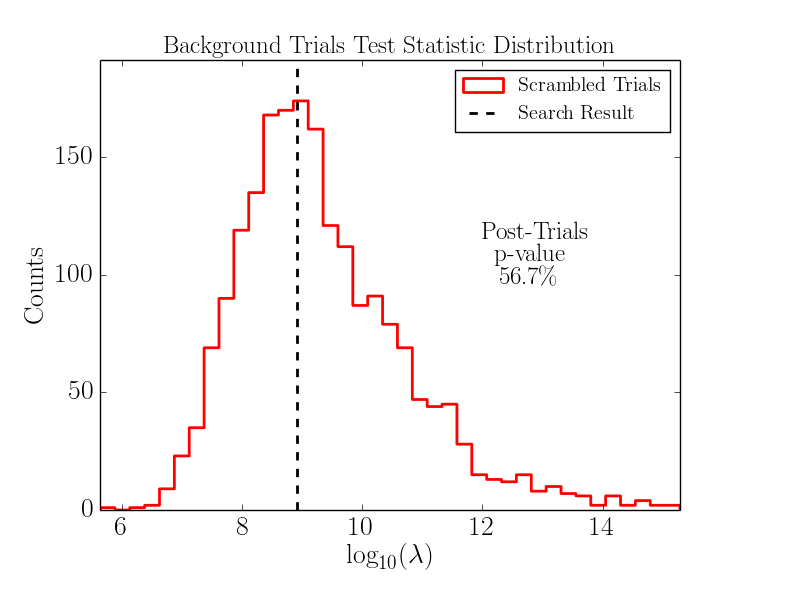
\includegraphics[width=1.0\textwidth,keepaspectratio]{TestStatisticDistribution_WithResult.png}
  \end{center}
  \caption{Distribution of test statistic $\lambda$ of most signficant flare found in 1,985 background trials. The test statistic value for the best fit flare on the unscrambled data set is also plotted.}
  \label{fig:RealSkyMap}
\end{figure}

\chapter{Interpretation}

%%Limits on Choked GRB fluence


%%
\chapter{Conclusion}

\appendix
\chapter{Appendix A -- Final Level Event Distributions}

%Ancillary material should be put in appendices, which 
%appear just before the bibliography. 

\begin{postliminary}
\bibliography{jdthesis}{}

\postfacesection{Index}{%
%%             ... generate an index here
%%         look into gatech-thesis-index.sty
}
\begin{vita}

\end{vita}
\end{postliminary}
\end{document}
